


% Use only LaTeX2e, calling the article.cls class and 12-point type.

\documentclass[12pt]{article}

% Users of the {thebibliography} environment or BibTeX should use the
% scicite.sty package, downloadable from *Science* at
% www.sciencemag.org/about/authors/prep/TeX_help/ .
% This package should properly format in-text
% reference calls and reference-list numbers.

\usepackage{scicite}

% Use times if you have the font installed; otherwise, comment out the
% following line.

\usepackage{times}

% The preamble here sets up a lot of new/revised commands and
% environments.  It's annoying, but please do *not* try to strip these
% out into a separate .sty file (which could lead to the loss of some
% information when we convert the file to other formats).  Instead, keep
% them in the preamble of your main LaTeX source file.


% The following parameters seem to provide a reasonable page setup.

\topmargin 0.0cm
\oddsidemargin 0.2cm
\textwidth 16cm
\textheight 21cm
\footskip 1.0cm


\usepackage{amsfonts}
\usepackage{graphicx}
\usepackage{epsfig}
\usepackage{epsf}
\usepackage{amssymb}
\usepackage{amsmath}
\usepackage{amsthm}
\usepackage{multirow}


\newcommand{\be}{\begin{equation}}
\newcommand{\ee}{\end{equation}}
\newcommand{\bea}{\begin{eqnarray}}
\newcommand{\eea}{\end{eqnarray}}
\newcommand{\Fig}[1]{Fig.\,\ref{#1}}
\newcommand{\Eq}[1]{Eq.\,(\ref{#1})}
\newcommand{\la}{\langle}
\newcommand{\ra}{\rangle}
\newcommand{\nl}{\nonumber \\}
%The next command sets up an environment for the abstract to your paper.

\newenvironment{sciabstract}{%
\begin{quote} \bf}
{\end{quote}}


% If your reference list includes text notes as well as references,
% include the following line; otherwise, comment it out.

%\renewcommand\refname{References and Notes}

% The following lines set up an environment for the last note in the
% reference list, which commonly includes acknowledgments of funding,
% help, etc.  It's intended for users of BibTeX or the {thebibliography}
% environment.  Users who are hand-coding their references at the end
% using a list environment such as {enumerate} can simply add another
% item at the end, and it will be numbered automatically.

\newcounter{lastnote}
\newenvironment{scilastnote}{%
\setcounter{lastnote}{\value{enumiv}}%
\addtocounter{lastnote}{+1}%
\begin{list}%
{\arabic{lastnote}.}
{\setlength{\leftmargin}{.22in}}
{\setlength{\labelsep}{.5em}}}
{\end{list}}


% Include your paper's title here

\title{Parameters of a 12-qubit NMR system}


% Place the author information here.  Please hand-code the contact
% information and notecalls; do *not* use \footnote commands.  Let the
% author contact information appear immediately below the author names
% as shown.  We would also prefer that you don't change the type-size
% settings shown here.

%\author
%{Dawei Lu,$^{1}$ Nanyang Xu,$^{1}$ Ruixue Xu,$^{1}$ Hongwei Chen,$^{1}$\\
% Xinhua Peng,$^{1}$ Jiangfeng Du,$^{1\ast}$\\
%\\
%\normalsize{$^{1}$Hefei National Laboratory for Physical Sciences at
%Microscale and Department of Modern Physics,} \\
%\normalsize{University of Science
%and Technology of China,}\\
%\normalsize{Hefei, Anhui 230026, People's Republic of
%China}\\
%\normalsize{$^\ast$To whom correspondence should be addressed; E-mail:  djf@ustc.edu.cn}
%}

% Include the date command, but leave its argument blank.

\date{}



%%%%%%%%%%%%%%%%% END OF PREAMBLE %%%%%%%%%%%%%%%%



\begin{document}

% Double-space the manuscript.

\baselineskip24pt

% Make the title.

\maketitle



% Place your abstract within the special {sciabstract} environment.

%\begin{sciabstract}
%  Exact simulations on quantum dynamics, using the present classical computers,
%are only limited to small systems and would become extremely expensive for large degrees of freedom.
%Quantum algorithms, on the other way, could be performed to simulate quantum systems using a moderate
%amount of resources, \emph{i.e.}, with a polynomial complexity.
%In this work we demonstrate the quantum simulation of a chemical
%isomerization reaction model system
%from a reactant state to a near-degenerate product state is simulated
%on a 3-qubit NMR (nuclear magnetic resonance) quantum computer.
%Firstly we discretized the reaction system with mapping it into the qubits' Hilbert space.
%Then we prepared the ground state of the reactant
%and let it propagate
%under an external field drive to the product state.
%Finally we measured the transition probability of the reaction.
%Although presented here is a simple demonstration,
%long-term applications with quantum computers of tens of qubits
%will no doubt surpass the capability of classical computers.


%\end{sciabstract}


% In setting up this template for *Science* papers, we've used both
% the \section* command and the \paragraph* command for topical
% divisions.  Which you use will of course depend on the type of paper
% you're writing.  Review Articles tend to have displayed headings, for
% which \section* is more appropriate; Research Articles, when they have
% formal topical divisions at all, tend to signal them with bold text
% that runs into the paragraph, for which \paragraph* is the right
% choice.  Either way, use the asterisk (*) modifier, as shown, to
% suppress numbering.

\section{Sample}

The 12-qubit NMR sample used in the experiment is $^{13}$C-labeled C$_7$H$_6$Cl$_2$SO$_3$, with the molecular structure shown in Fig. \ref{para}.
\begin{figure}[h] \centering
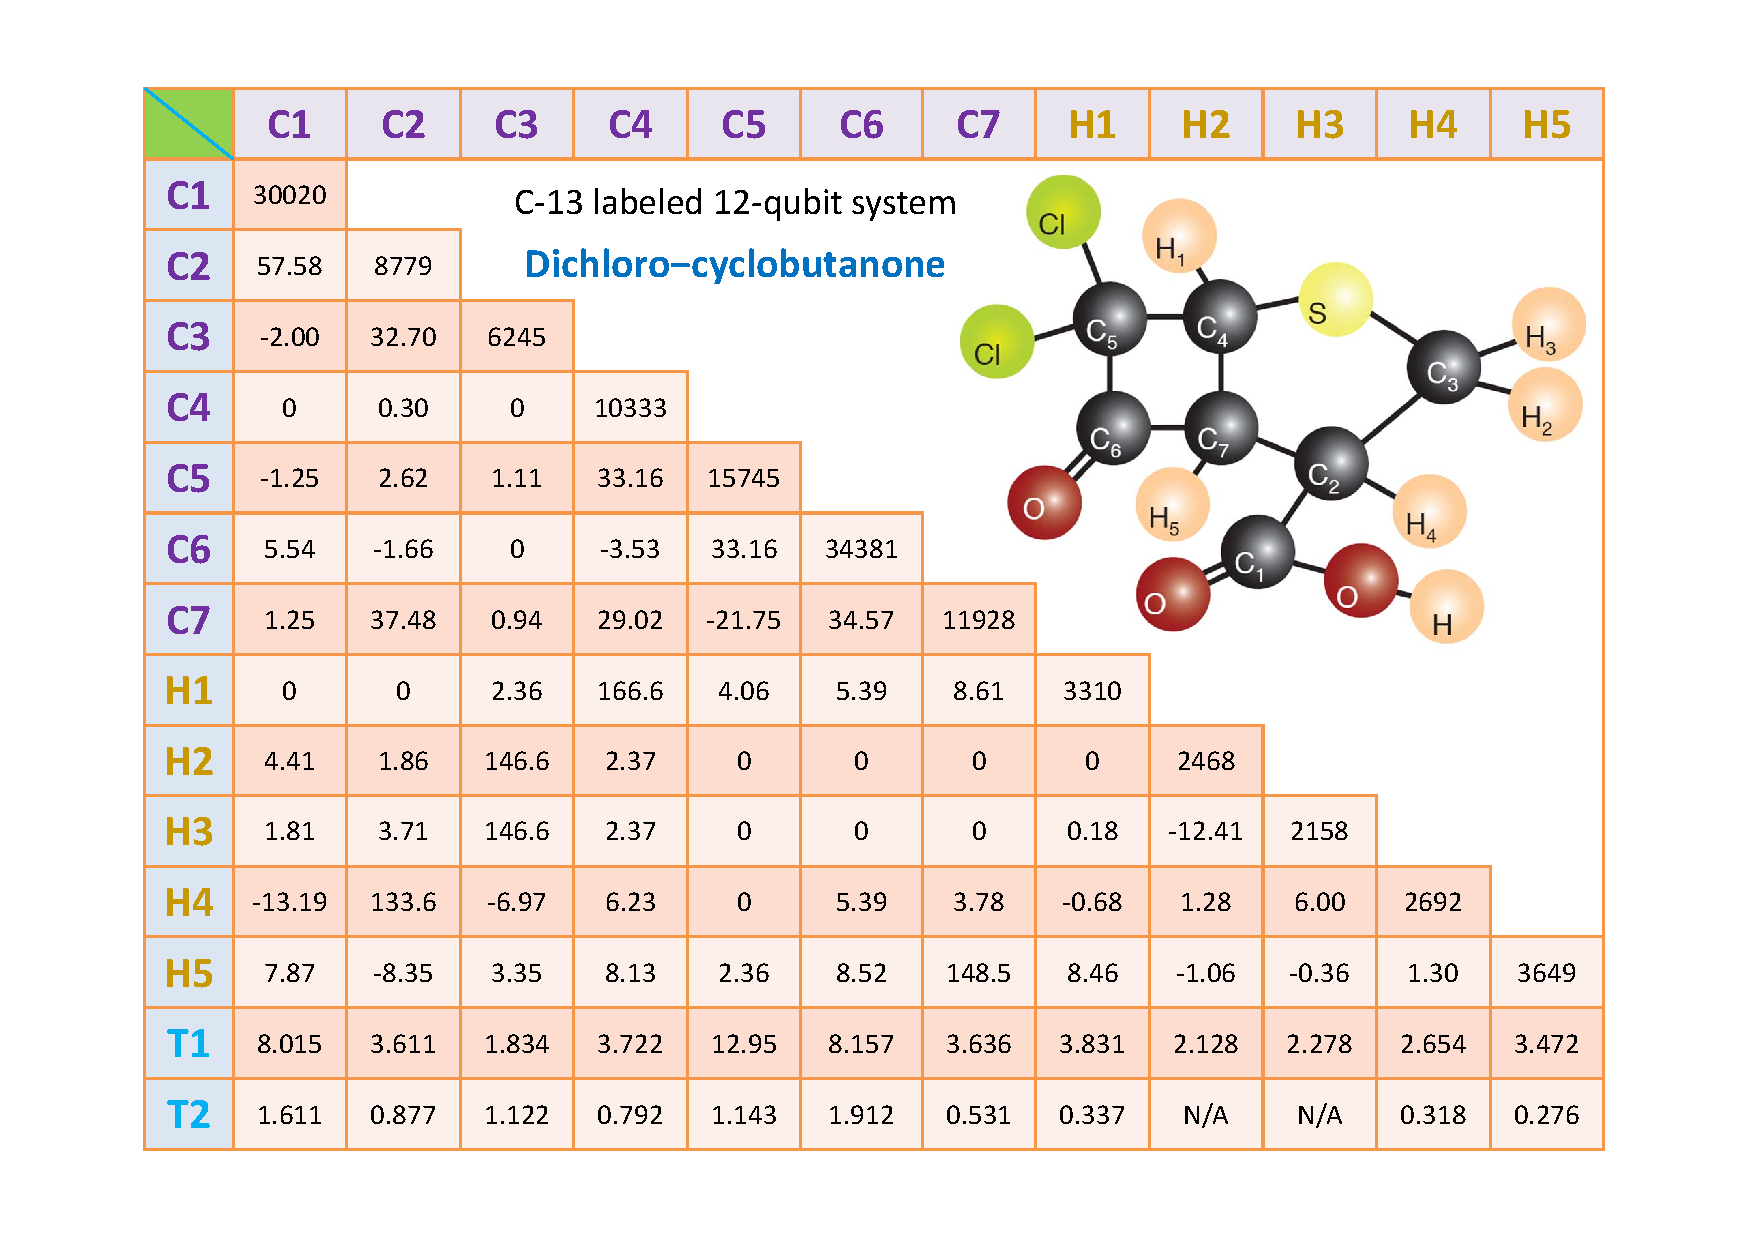
\includegraphics[width=0.9\columnwidth]{parax_new.pdf}
\caption{System parameters of the C$_7$H$_6$Cl$_2$SO$_3$ molecule. The diagonal elements are chemical shifts (Hz), and the lower-left off-diagonal elements are scalar coupling strengths (Hz). The molecular structure is shown in the upper-right part of the table.}\label{para}
\end{figure}
Approximately 20mg of the sample was dissolved in 1mL of Acetone-d6. The internal Hamiltonian of this system can be described as
\begin{eqnarray}\label{Hamiltonian}
\mathcal{H}_{int}=&&\sum\limits_{j=1}^{12} {2\pi \nu _j } I_z^j  + \sum\limits_{j < k,=1}^{12} {2\pi} J_{jk} I_z^j I_z^k,
\end{eqnarray}
where $\nu _j$ is the resonant frequency of the \emph{j}th spin and $\emph{J}_{jk}$ is the scalar coupling strength between spins \emph{j} and
\emph{k}. The experiment is conducted on a Bruker Avance 700 MHz spectrometer at room temperature.

Although a weakly coupled spin system, the NMR spectra of this large system are still very complicated, as there are about eleven interactions for every nucleus. Fig. \ref{thermal_c} and Fig. \ref{thermal_h} show the spectra of the thermal equilibrium for $^{13}$C and $^{1}$H, respectively.
\begin{figure}[h] \centering
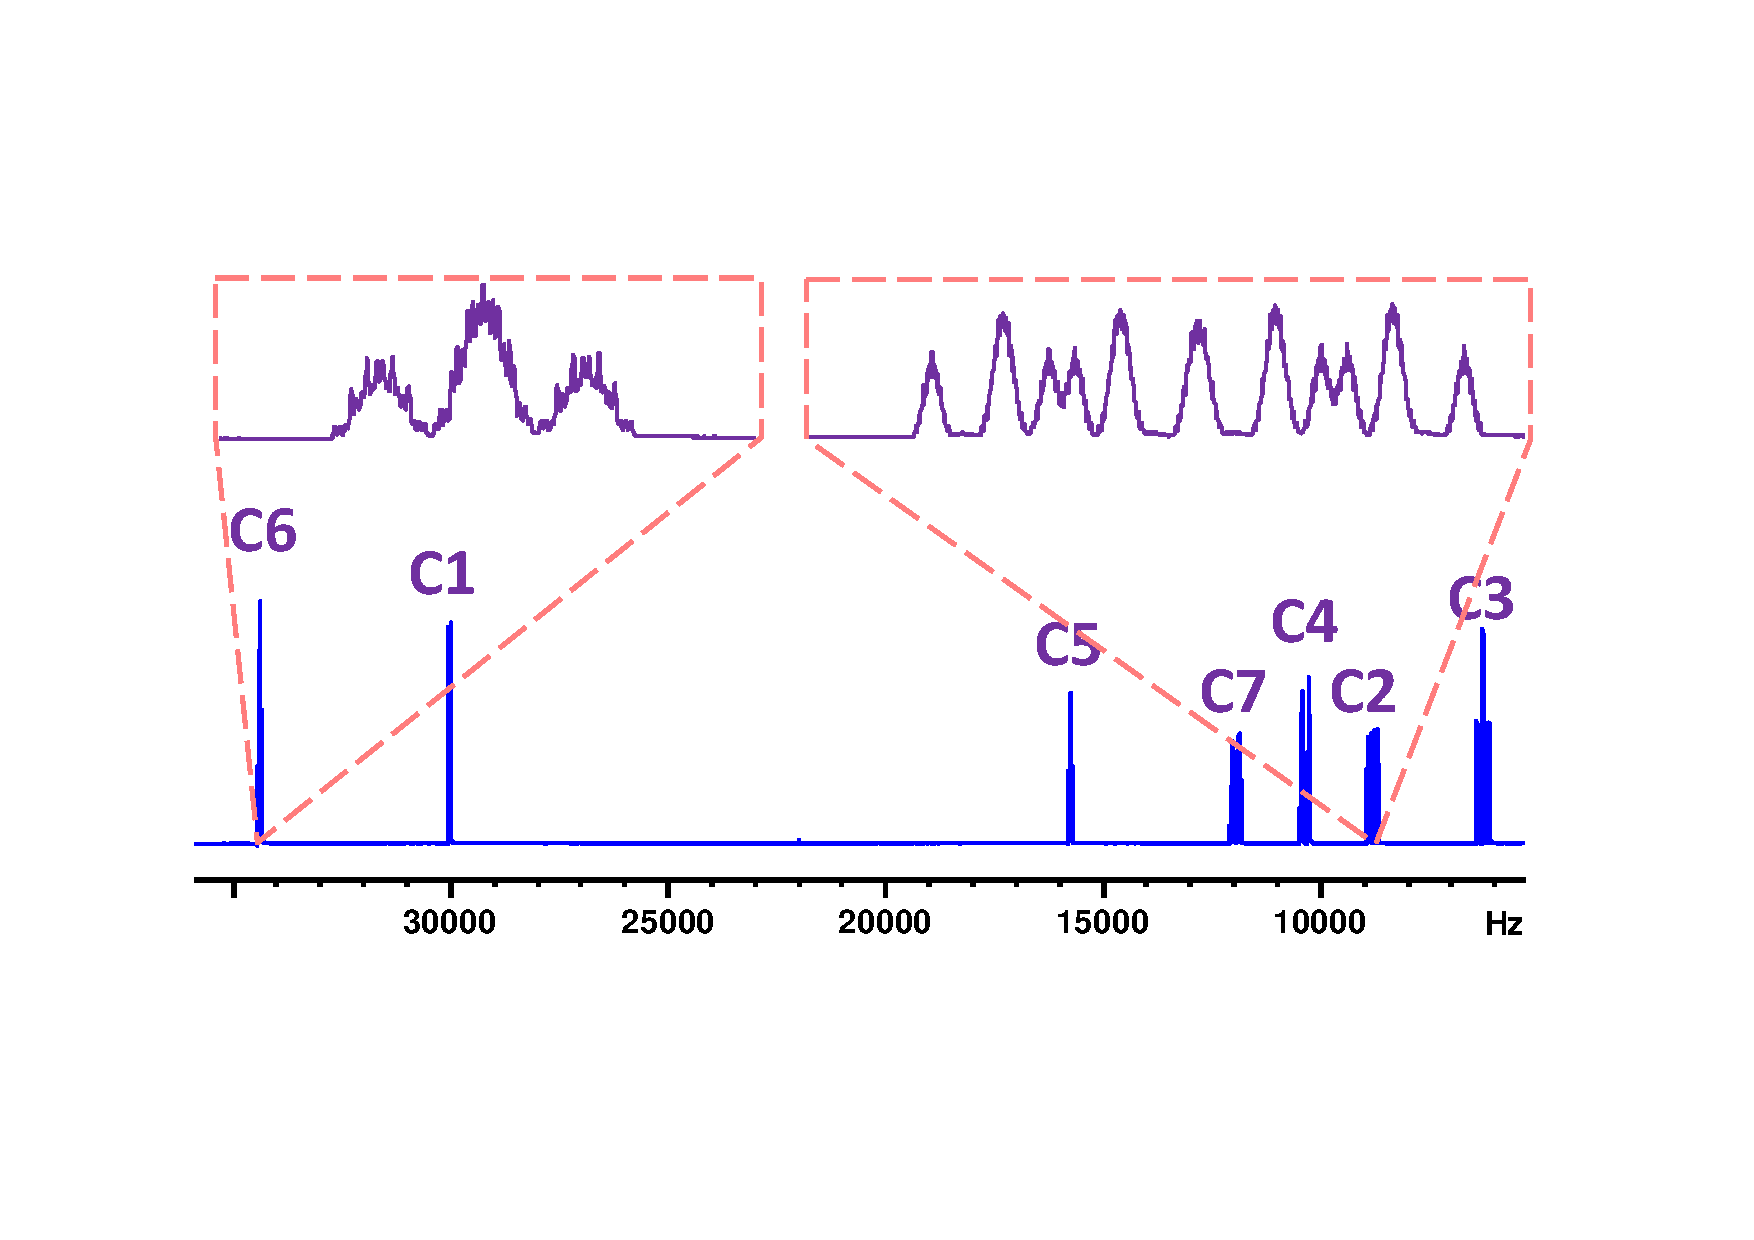
\includegraphics[width=0.9\columnwidth]{thermal_c.pdf}
\caption{Spectrum of the thermal equilibrium state followed by a $\pi/2$ hard pulse in the $^{13}$C channel, with the pulse width 14.94$\mu$s. The two channels of $^{13}$C and $^{1}$H are not decoupled here.}\label{thermal_c}
\end{figure}
\begin{figure}[h] \centering
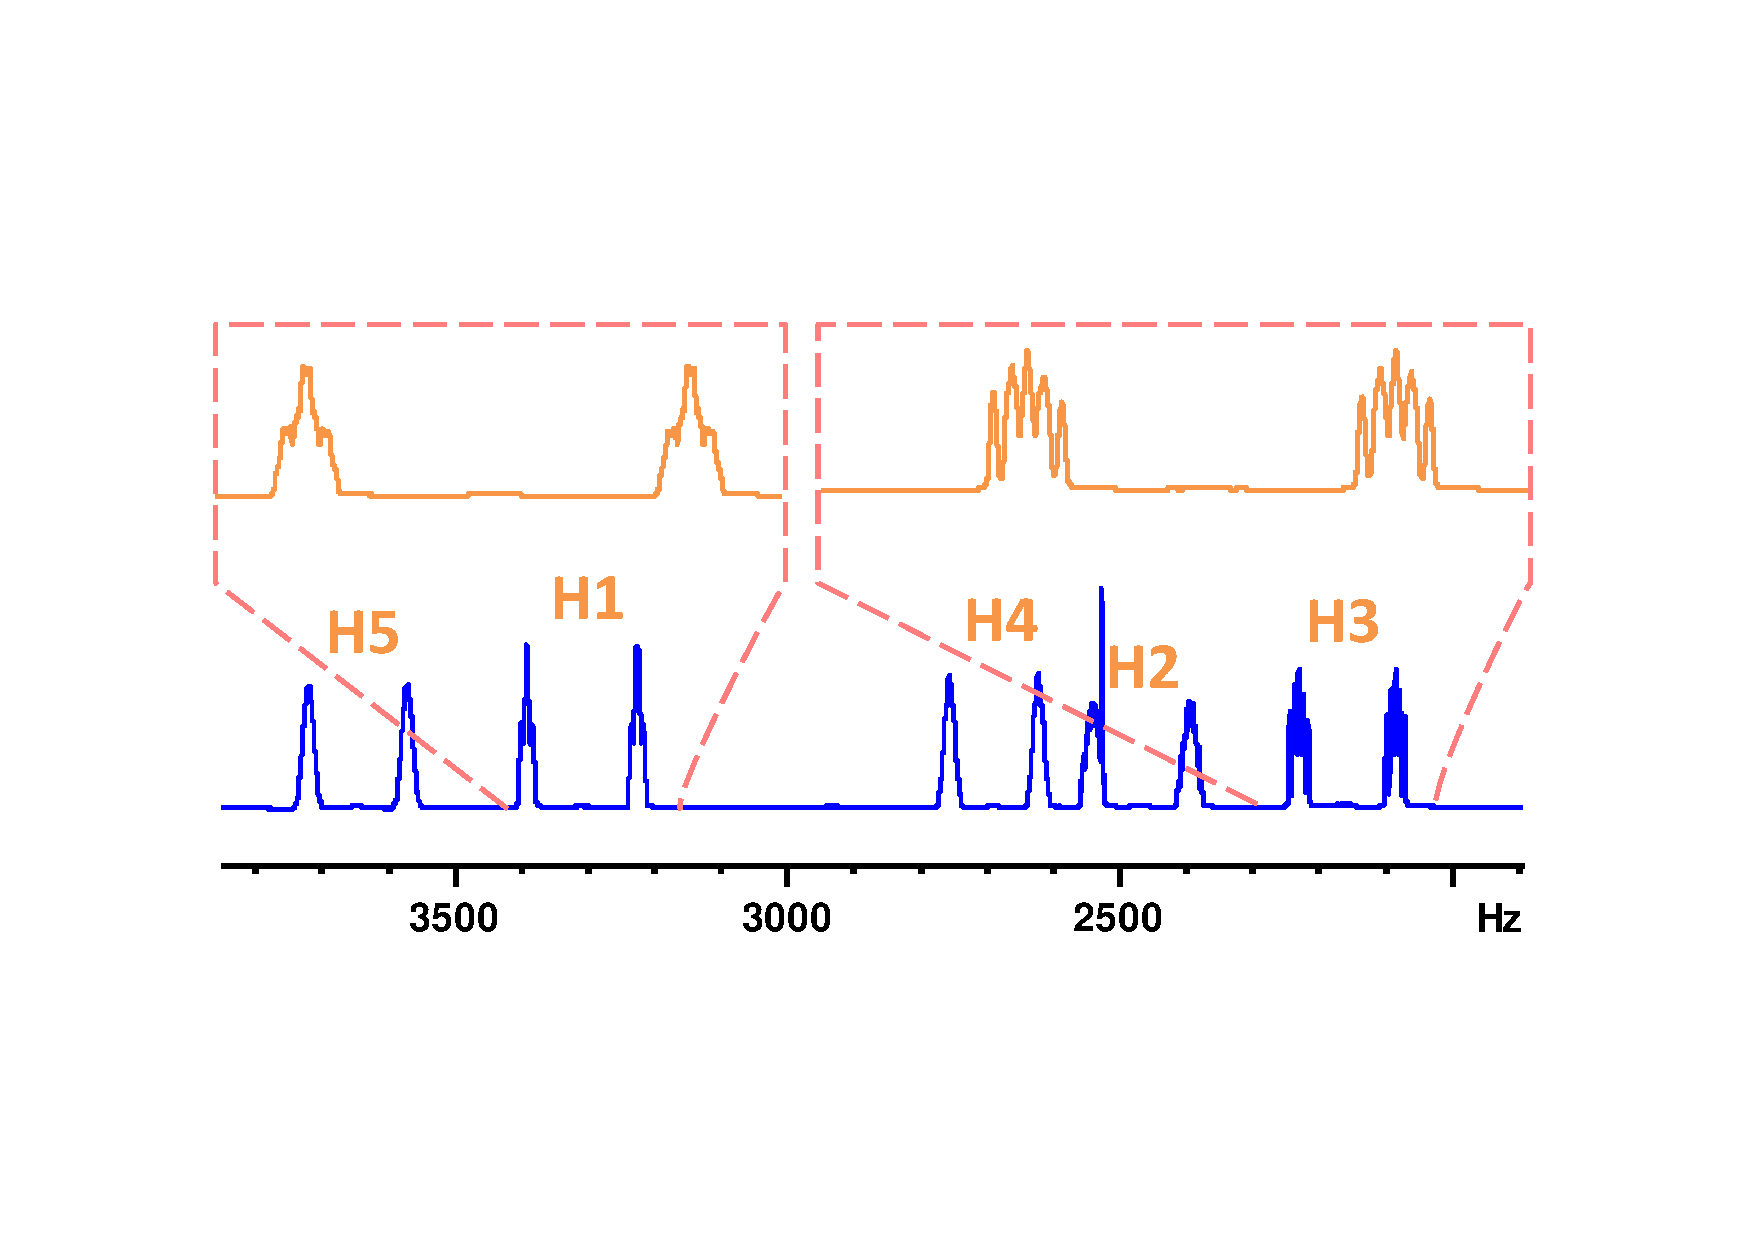
\includegraphics[width=0.9\columnwidth]{thermal_h.pdf}
\caption{Spectrum of the thermal equilibrium state followed by a $\pi/2$ hard pulse in the $^{1}$H channel, with the pulse width 8.8$\mu$s. The two channels of $^{13}$C and $^{1}$H are not decoupled here.}\label{thermal_h}
\end{figure}

\section{Magnitude of the Homonuclear J-Couplings}

For measuring the magnitudes of the homonuclear J-couplings, we used 2D J-resolved NMR technique. The pulse sequence in the experiment is the conventional 2D spin-echo sequence (Fig. \ref{jresolved}(b)). Without loss of generality, we choose the experiment of measuring $^{1}$H homonuclear J-couplings here. Because one $\pi$ pulse is inserted in the middle of t1-evolution, the chemical shifts of all the protons and the heteronuclear J-couplings are both completely refocused. Therefore, the projection on F1 dimension (\emph{y}-axis in the 2D spectrum in Fig. \ref{jresolved}(a)) only  involves the homonuclear J-couplings. Meanwhile, the projection on F2 dimension (\emph{x}-axis in the 2D spectrum in Fig. \ref{jresolved}(a)) is the thermal equilibrium spectrum. By projecting the region of each proton on F1 dimension, we can obtain the corresponding spectrum for the proton, which just contains the homonuclear J-couplings.
\begin{figure}[h] \centering
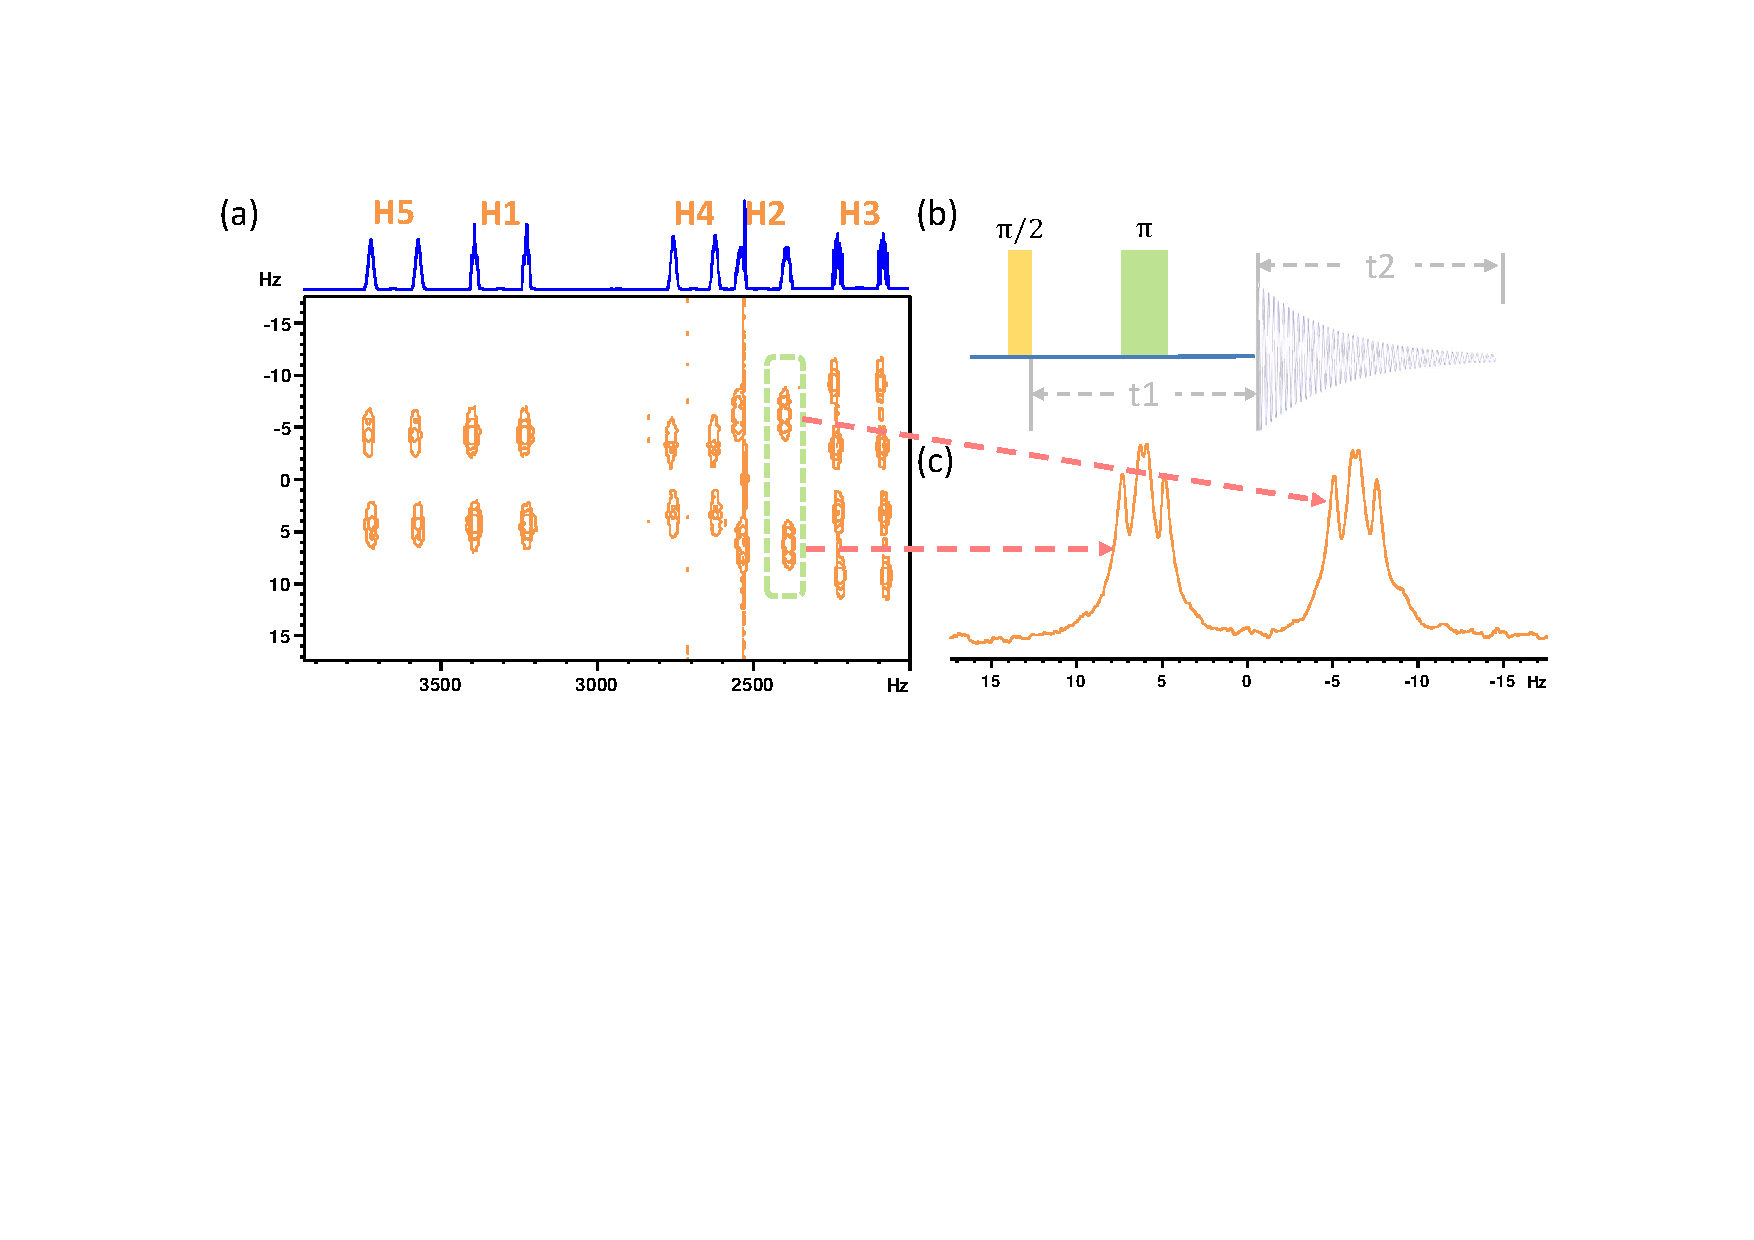
\includegraphics[width=0.9\columnwidth]{jresolved.pdf}
\caption{Spin-echo J-resolved 2D experiment for $^{1}$H channel. (a)Full 2D proton spectrum showing the heteronuclear J-couplings in the cross section parallel to F2 (\emph{x}-axis) and the homonuclear J-couplings parallel to F1 (\emph{y}-axis). (b) Pulse sequence of the J-resolved 2D experiment. (c) Projection of H2 nucleus on F1 dimension, which just shows homonuclear J-couplings.}\label{jresolved}
\end{figure}

\section{Sign of the Homonuclear J-Couplings}
The signs of the Homonuclear J-Couplings can be determined using 2D COSY45 experiment. From the pulse sequence shown in Fig. \ref{cosy45}(a), we can see that the projections on F1 and F2 dimension both give the thermal equilibrium spectra. However, in 2D experiment, the directions of the selected region corresponding to two protons are different (Fig. \ref{cosy45}(b)). If the direction is parallel to the diagonal, the sign of the relative protons is negative; otherwise the sign is positive. The two rectangles in Fig. \ref{cosy45}(b) display that the sign of J$_{\texttt{H}4\texttt{H}5}$ is positive, and the sign of J$_{\texttt{H}1\texttt{H}4}$ is negative, respectively.
\begin{figure}[h] \centering
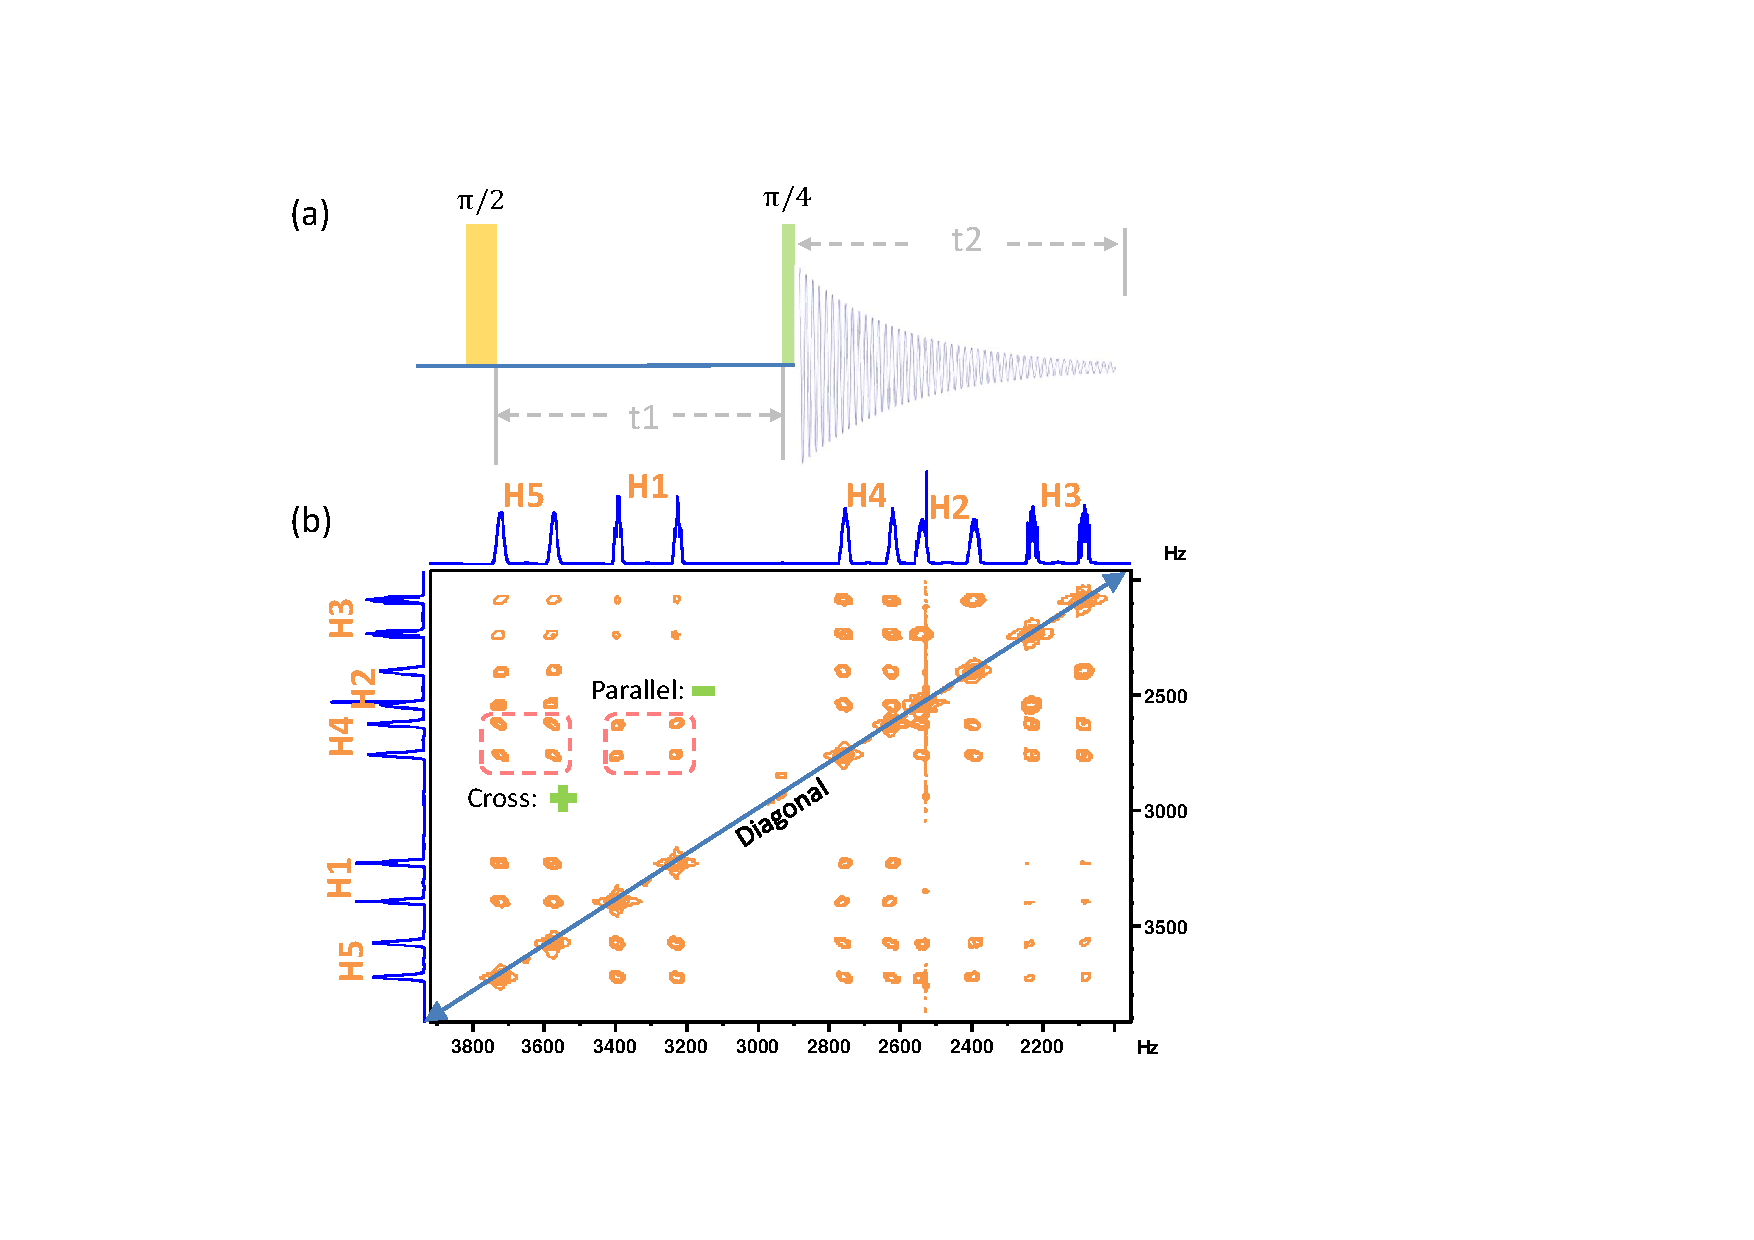
\includegraphics[width=0.9\columnwidth]{cosy45.pdf}
\caption{COSY45 2D experiment for $^{1}$H channel. (a)Pulse sequence of the COSY45 2D experiment. (b)Full 2D proton spectrum showing the signs of the homonuclear J-couplings. The direction parallel to the diagonal represents the relative J-coupling is positive, while the direction unparallel represents negative.}\label{cosy45}
\end{figure}
% Your references go at the end of the main text, and before the
% figures.  For this document we've used BibTeX, the .bib file
% scibib.bib, and the .bst file Science.bst.  The package scicite.sty
% was included to format the reference numbers according to *Science*
% style.

\clearpage

\section{Appendix}

\subsection{2D-COSY45 Experiment}

2D-COSY(Correlation Spectroscopy) is a basic but important 2D NMR technique. The universal pulse sequence of COSY is shown in Fig. \ref{cosy}(a). As a simple example, firstly we consider the two-spin system, with the internal Hamiltonian
\begin{eqnarray}\label{2Hamil}
\mathcal{H}_{int}= \omega_1 I_z^1+\omega_2 I_z^2 + 2\pi J I_z^1 I_z^2.
\end{eqnarray}
$\omega_1 = 2\pi\nu_1, \omega_2 = 2\pi\nu_2.$ $\nu_1$ and $\nu_2$ are chemical shifts of spin 1 and 2, respectively. If we apply the COSY sequence to this system from the thermal equilibrium state $\sigma_0 = I_z^1 + I_z^2$, the state of point 1 will be $\sigma_1 = -I_y^1 - I_y^2$ through simple calculation. Under the free evolution time $t_1$, the state of point 2 is
\begin{eqnarray}\label{2Hamil}
\sigma_2 & = &-[I_y^1cos\omega_1 t_1 + I_y^2 cos\omega_2 t_1]cos\pi J t_1 + [I_x^1sin\omega_1 t_1 + I_x^2 sin\omega_2 t_1]cos\pi J t_1 \\ \nonumber
&&+[2I_x^1I_z^2cos\omega_1 t_1 + I_z^2I_x^1 cos\omega_2 t_1]sin\pi J t_1+[2I_y^1I_z^2sin\omega_1 t_1 + I_z^2I_y^1 sin\omega_2 t_1]sin\pi J t_1.
\end{eqnarray}
After applying a $R_x(\beta)$ on $\sigma_2$, the final state of the COSY sequence will be
\begin{eqnarray}\label{2Hamil}
\sigma_3 & = &-[I_z^1cos\omega_1 t_1 + I_z^2 cos\omega_2 t_1]cos\pi J t_1sin \beta \\ \nonumber
&&+ [I_x^1sin\omega_1 t_1 + I_x^2 sin\omega_2 t_1]cos\pi J t_1 \\ \nonumber
&&-[I_y^1cos\omega_1 t_1 + I_y^2 cos\omega_2 t_1]cos\pi J t_1cos \beta \\ \nonumber
&&+ [2I_z^1I_z^2sin\omega_1 t_1 + 2I_z^1I_z^2 sin\omega_2 t_1]sin\pi J t_1 sin\beta cos\beta\\ \nonumber
&&+[2I_x^1I_z^2cos\omega_1 t_1 + 2I_z^2I_x^1 cos\omega_2 t_1]sin\pi J t_1cos\beta \\ \nonumber
&&+[2I_y^1I_z^2sin\omega_1 t_1 + 2I_z^1I_y^2 sin\omega_2 t_1]sin\pi J t_1cos^2\beta \\ \nonumber
&&-[2I_z^1I_y^2sin\omega_1 t_1 + 2I_y^1I_z^2 sin\omega_2 t_1]sin\pi J t_1 sin^2\beta \\ \nonumber
&&-[2I_x^1I_y^2cos\omega_1 t_1 + 2I_y^1I_x^2 cos\omega_2 t_1]sin\pi J t_1 sin\beta\\ \nonumber
&&-[2I_y^1I_y^2sin\omega_1 t_1 + 2I_y^1I_y^2 sin\omega_2 t_1]sin\pi J t_1 sin\beta.
\end{eqnarray}
The most important term of this formula is $-[2I_z^1I_y^2sin\omega_1 t_1 + 2I_y^1I_z^2 sin\omega_2 t_1]sin\pi J t_1 sin^2\beta$, as it leads to the multiplet of  cross peaks. Without loss of generality, we could consider $-2I_z^1I_y^2sin\omega_1 t_1 sin\pi J t_1$ instead.

\begin{figure}[h] \centering
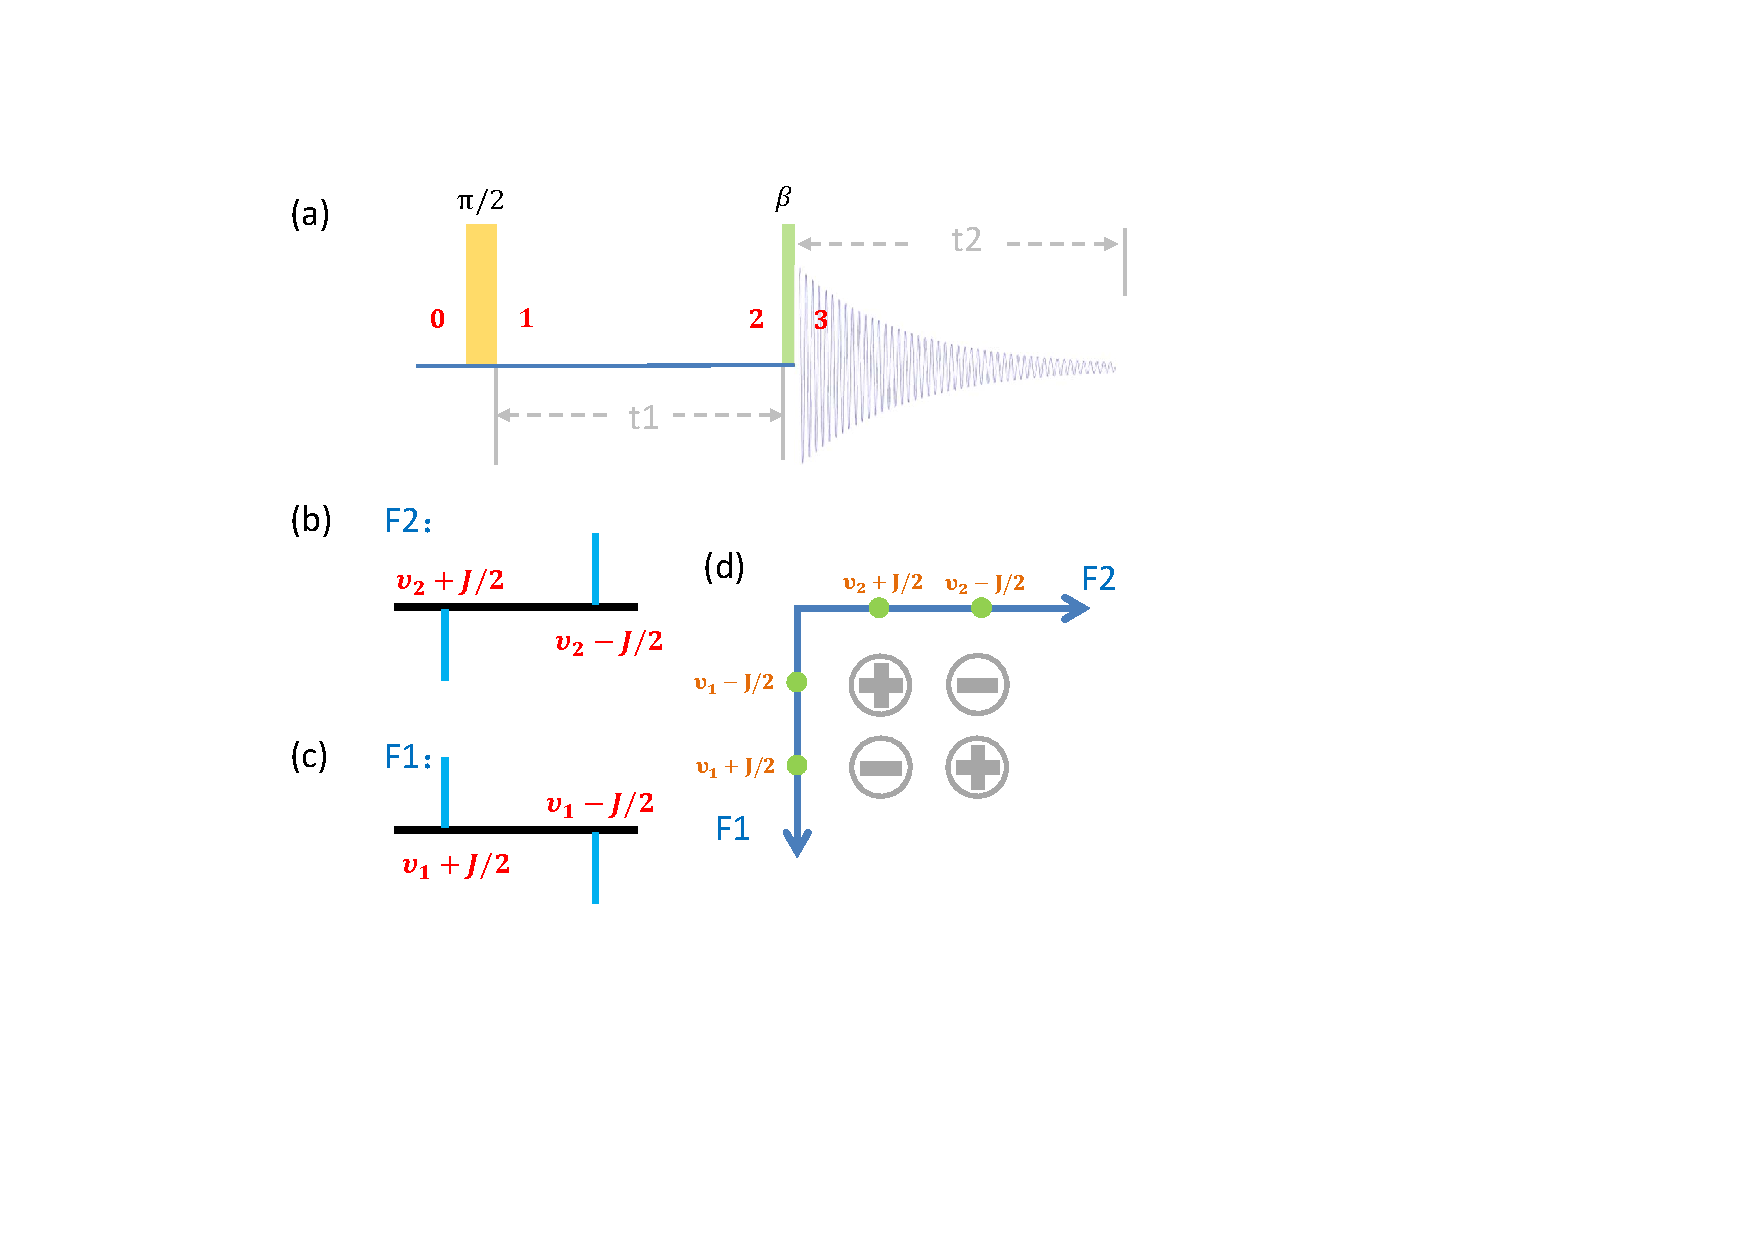
\includegraphics[width=0.9\columnwidth]{cosy.pdf}
\caption{(a)Pulse sequence of the COSY45 2D experiment. (b)Spectrum of the cross-peak term in F$_2$ dimension. (c)Spectrum of the cross-peak term in F$_1$ dimension. (d) 2D spectrum of the cross-peak multiplet.}\label{cosy}
\end{figure}

First, implement Fourier Transform of $t_2$, which results the spectra in F$_2$ domain. The part that contributes to the F$_2$ domain is $-2I_z^1I_y^2$. It has two antiphase peaks, with the negative one at the frequency $\nu_2+J/2$ and the positive one at the frequency $\nu_2-J/2$.
Hereafter we use $-A_{2+}$ and $+A_{2-}$ to represent the two cases. The left sign stands for the phase of the peak, $A$ means "antiphase", and $2+$ and $2-$ stand for the positions of peaks. Fig. \ref{cosy}(b) shows a schematic 1D spectrum.

Then, implement Fourier Transform of $t_1$, which results the spectra in F$_1$ domain. Note that the part that contributes to the Fourier Transform is $sin\omega_1t_1 sin\pi J t_1$. It also has two antiphase peaks $+A_{1+}$ and $-A_{1-}$, meaning that the peak at $\nu_1+J/2$ is positive and the peak at $\nu_1-J/2$ is negative.

To obtain a 2D spectrum, we should combine the spectrum of $t_1$ and $t_2$, and calculate the product of the corresponding peaks. The multiplet of
the cross peaks is
\begin{eqnarray}\label{2Hamil}
-(A_{1+}A_{2+})+(A_{1-}A_{2+})+(A_{1+}A_{2-})-(A_{1-}A_{2-}),
\end{eqnarray}
and the schematic 2D spectrum is shown in Fig. \ref{cosy}(d). Obviously whenever $J>0$ or $J<0$, we cannot distinguish them through the 2D spectrum.

When the system is scaled to three spins whose Hamiltonian is
\begin{eqnarray}\label{2Hamil}
\mathcal{H}_{int}= \omega_1 I_z^1+\omega_2 I_z^2 +\omega_3 I_z^3+ 2\pi J_{12} I_z^1 I_z^2+2\pi J_{13} I_z^1 I_z^3+2\pi J_{23} I_z^2 I_z^3,
\end{eqnarray}
it is able to obtain the relative signs of the three couplings. Without loss of generality, we would consider the cross-peak multiplet of the 2D spectrum under the condition $|J_{12}|>|J_{23}|>|J_{13}|$, and all the couplings are positive.

In this case, after COSY sequence the term that will contribute to the cross peaks consists of two parts:
\begin{eqnarray}\label{2Hamil}
(i) -2I_z^1I_y^2sin\omega_1 t_1 sin\pi J_{12} t_1 cos\pi J_{13} t_1 sin^2\beta,
\end{eqnarray}
and
\begin{eqnarray}\label{2Hamil}
(ii) -4I_z^1I_y^2I_z^3 cos\omega_1 t_1 sin\pi J_{12} t_1 sin\pi J_{13} t_1 cos\beta sin^2\beta.
\end{eqnarray}

For (i), the part that would affect Fourier Transform of $t_2$ is $-2I_z^1I_y^2$, which will result the spectrum in F$_2$ domain as shown in Fig. \ref{3cosy}(a); the part that would affect Fourier Transform of $t_1$ is $sin\omega_1 t_1 sin\pi J_{12} t_1 cos\pi J_{13} t_1$, which will result the spectrum in F$_1$ domain as shown in Fig. \ref{3cosy}(b). Therefore, the cross peaks in the 2D spectrum display as Fig. \ref{3cosy}(c).

\begin{figure}[h] \centering
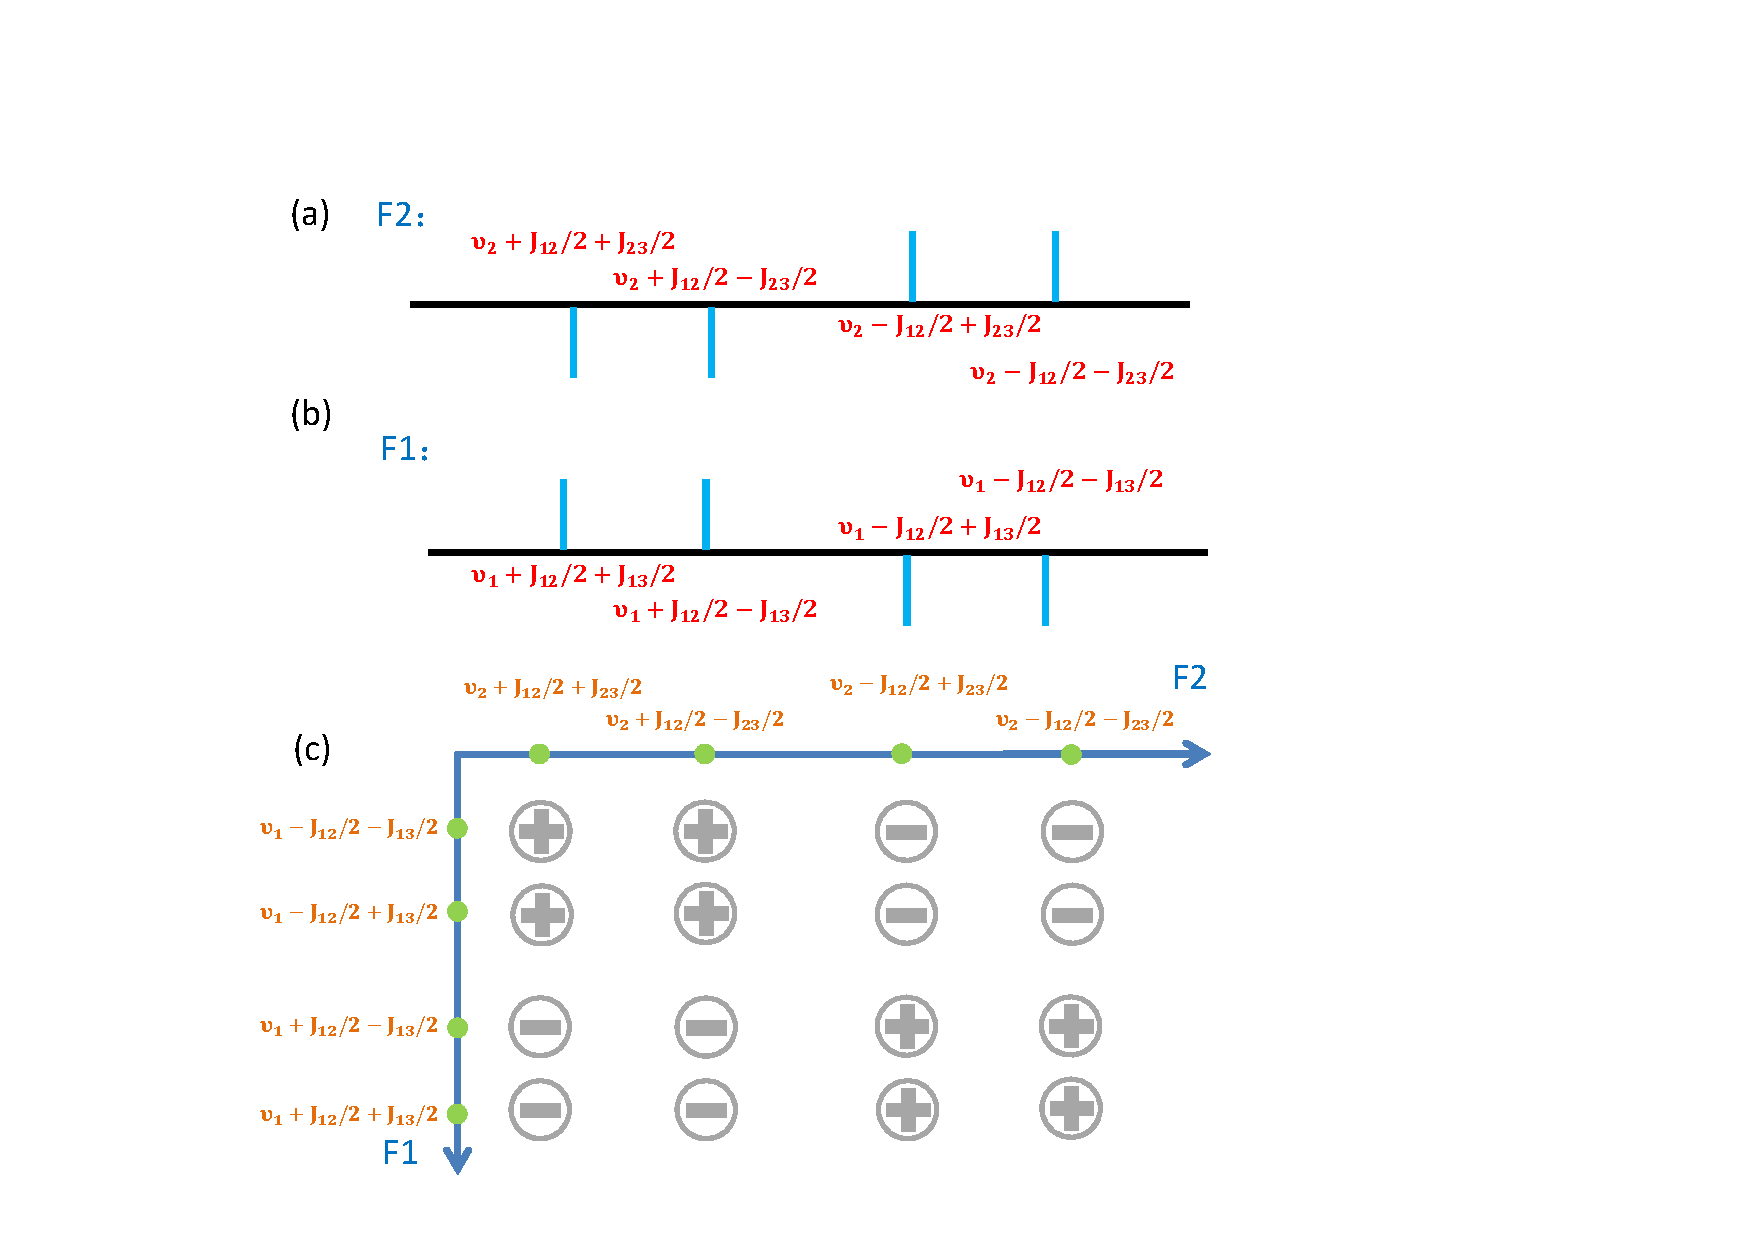
\includegraphics[width=0.9\columnwidth]{3cosy.pdf}
\caption{(a)Spectrum of term (i) in F$_2$ dimension. (b)Spectrum of term (i) in F$_1$ dimension. (c) 2D spectrum of the cross-peak multiplet.}\label{3cosy}
\end{figure}

For (ii), the part that would affect Fourier Transform of $t_2$ is $-4I_z^1I_y^2I_z^3$, which will result the spectrum in F$_2$ domain as shown in Fig. \ref{4cosy}(a); the part that would affect Fourier Transform of $t_1$ is $cos\omega_1 t_1 sin\pi J_{12} t_1 sin\pi J_{13} t_1 $, which will result the spectrum in F$_1$ domain as shown in Fig. \ref{4cosy}(b). Therefore, the cross peaks in the 2D spectrum display as Fig. \ref{4cosy}(c).

\begin{figure}[h] \centering
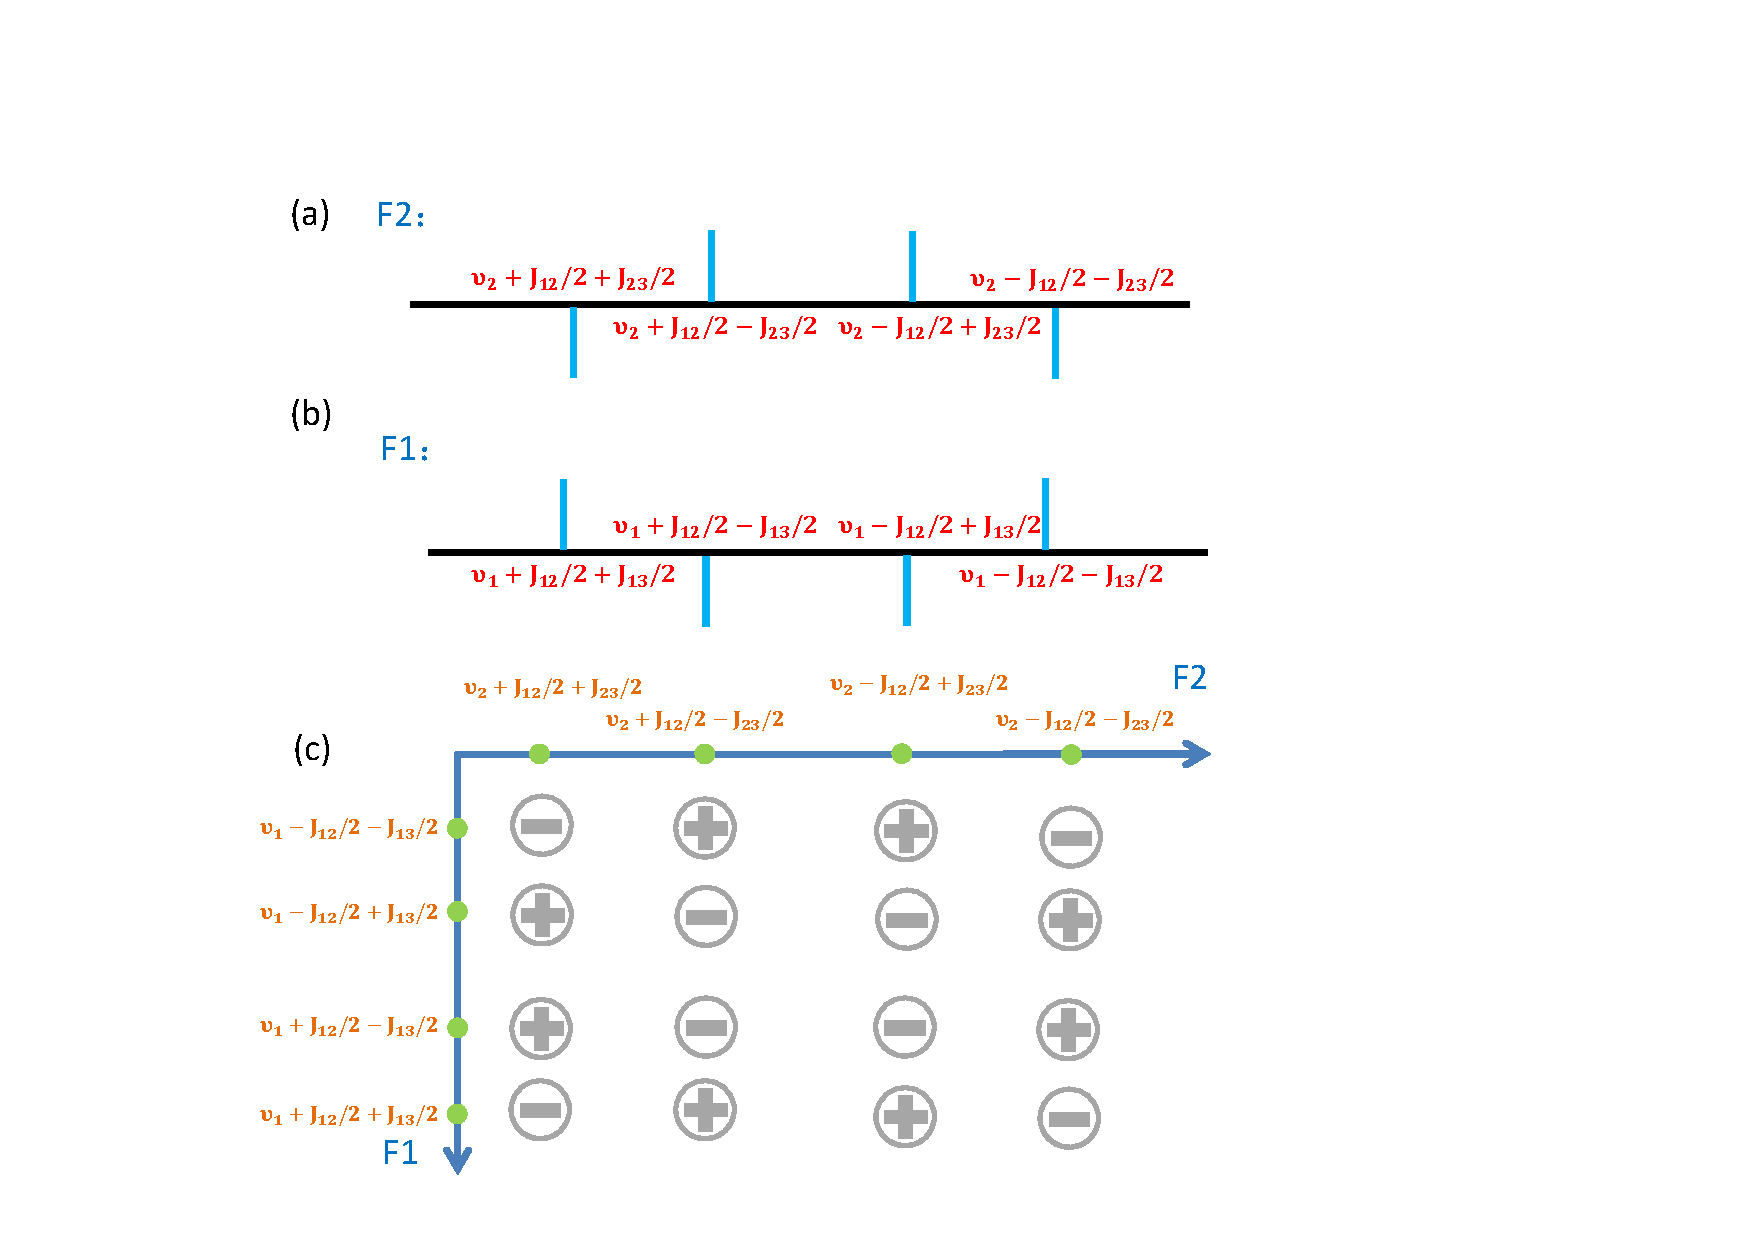
\includegraphics[width=0.9\columnwidth]{4cosy.pdf}
\caption{(a)Spectrum of term (ii) in F$_2$ dimension. (b)Spectrum of term (ii) in F$_1$ dimension. (c) 2D spectrum of the cross-peak multiplet.}\label{4cosy}
\end{figure}

The last step is adding Fig. \ref{3cosy}(c) and Fig. \ref{4cosy}(c) to get a final 2D spectrum. Noting that term (i) is weighted by $sin^2\beta$, while term (ii) is weighted by $cos\beta sin^2\beta$. If $\beta = \pi/4$, the strengths of some cross peaks will decrease and the strengths of the other cross peaks will increase. The whole result is that a positive tilt appears in the spectrum, as shown in Fig. \ref{allcosy}. In other words, a positive tilt demonstrates that $J_{13}$ and $J_{23}$ have the same signs.

Now suppose $J_{13}$ and $J_{23}$ have opposite signs, for example, $J_{13}<0$. It means that in F$_1$ dimension, we should exchange two pairs of lines: the lines of $\nu_1-J_{12}/2-J_{13}/2$ and $\nu_1-J_{12}/2+J_{13}/2$, and the lines of $\nu_1+J_{12}/2-J_{13}/2$ and $\nu_1+J_{12}/2+J_{13}/2$. This will produce a negative tilt, which is different from the case of same signs. Through the tilt direction of the cross peaks, we could infer the relative signs of $J_{13}$ and $J_{23}$.

\begin{figure}[h] \centering
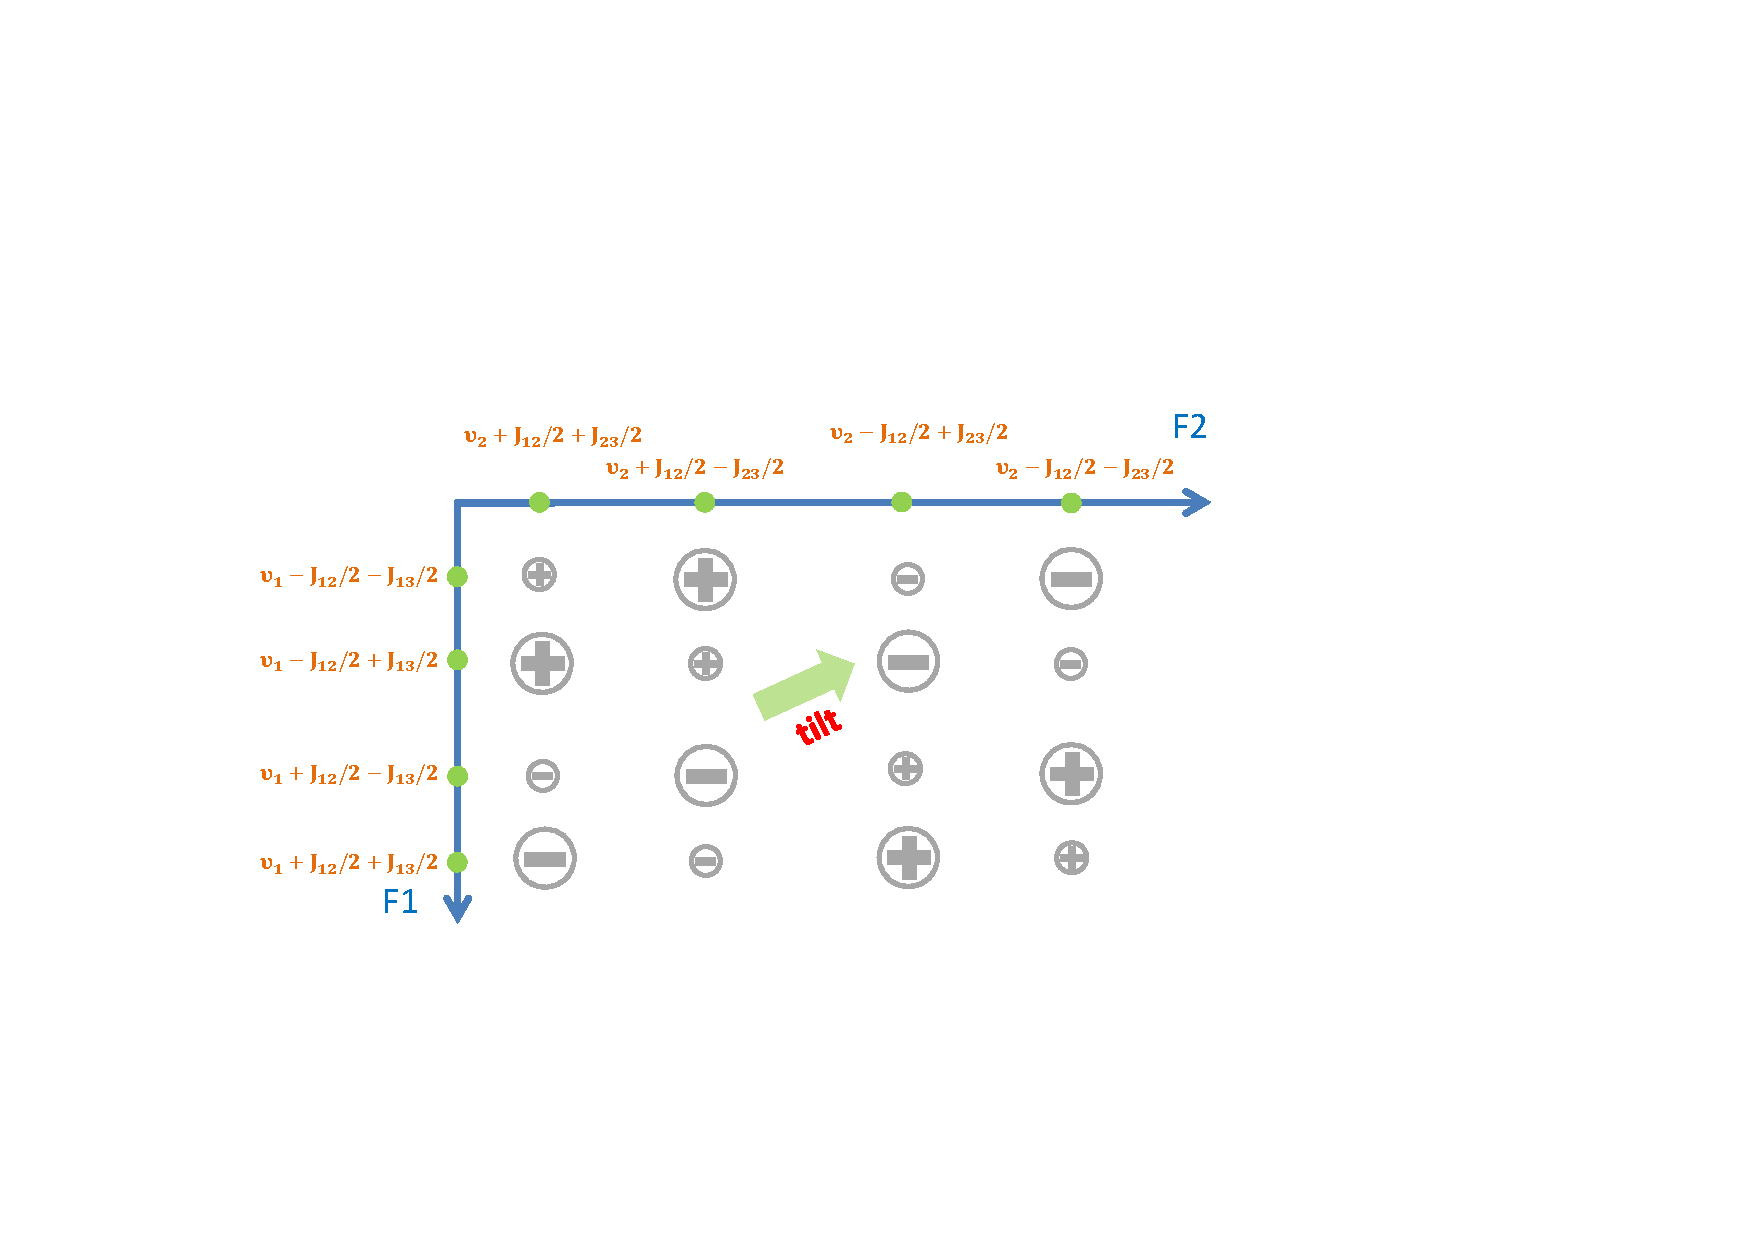
\includegraphics[width=0.9\columnwidth]{allcosy.pdf}
\caption{(a)Spectrum of term (ii) in F$_2$ dimension. (b)Spectrum of term (ii) in F$_1$ dimension. (c) 2D spectrum of the cross-peak multiplet.}\label{allcosy}
\end{figure}

\subsection{1D Experiment to Determine the relative signs of J-couplings}

Although intuitively, 2D COSY experiments still have a few disadvantages, e.g., long measurement time, big data for 2D spectra and incapable for small couplings. By 1D experiment, we could solve these problems more or less. The following is an example of how to determine the relative signs of a three-spin system.

\begin{figure}[h] \centering
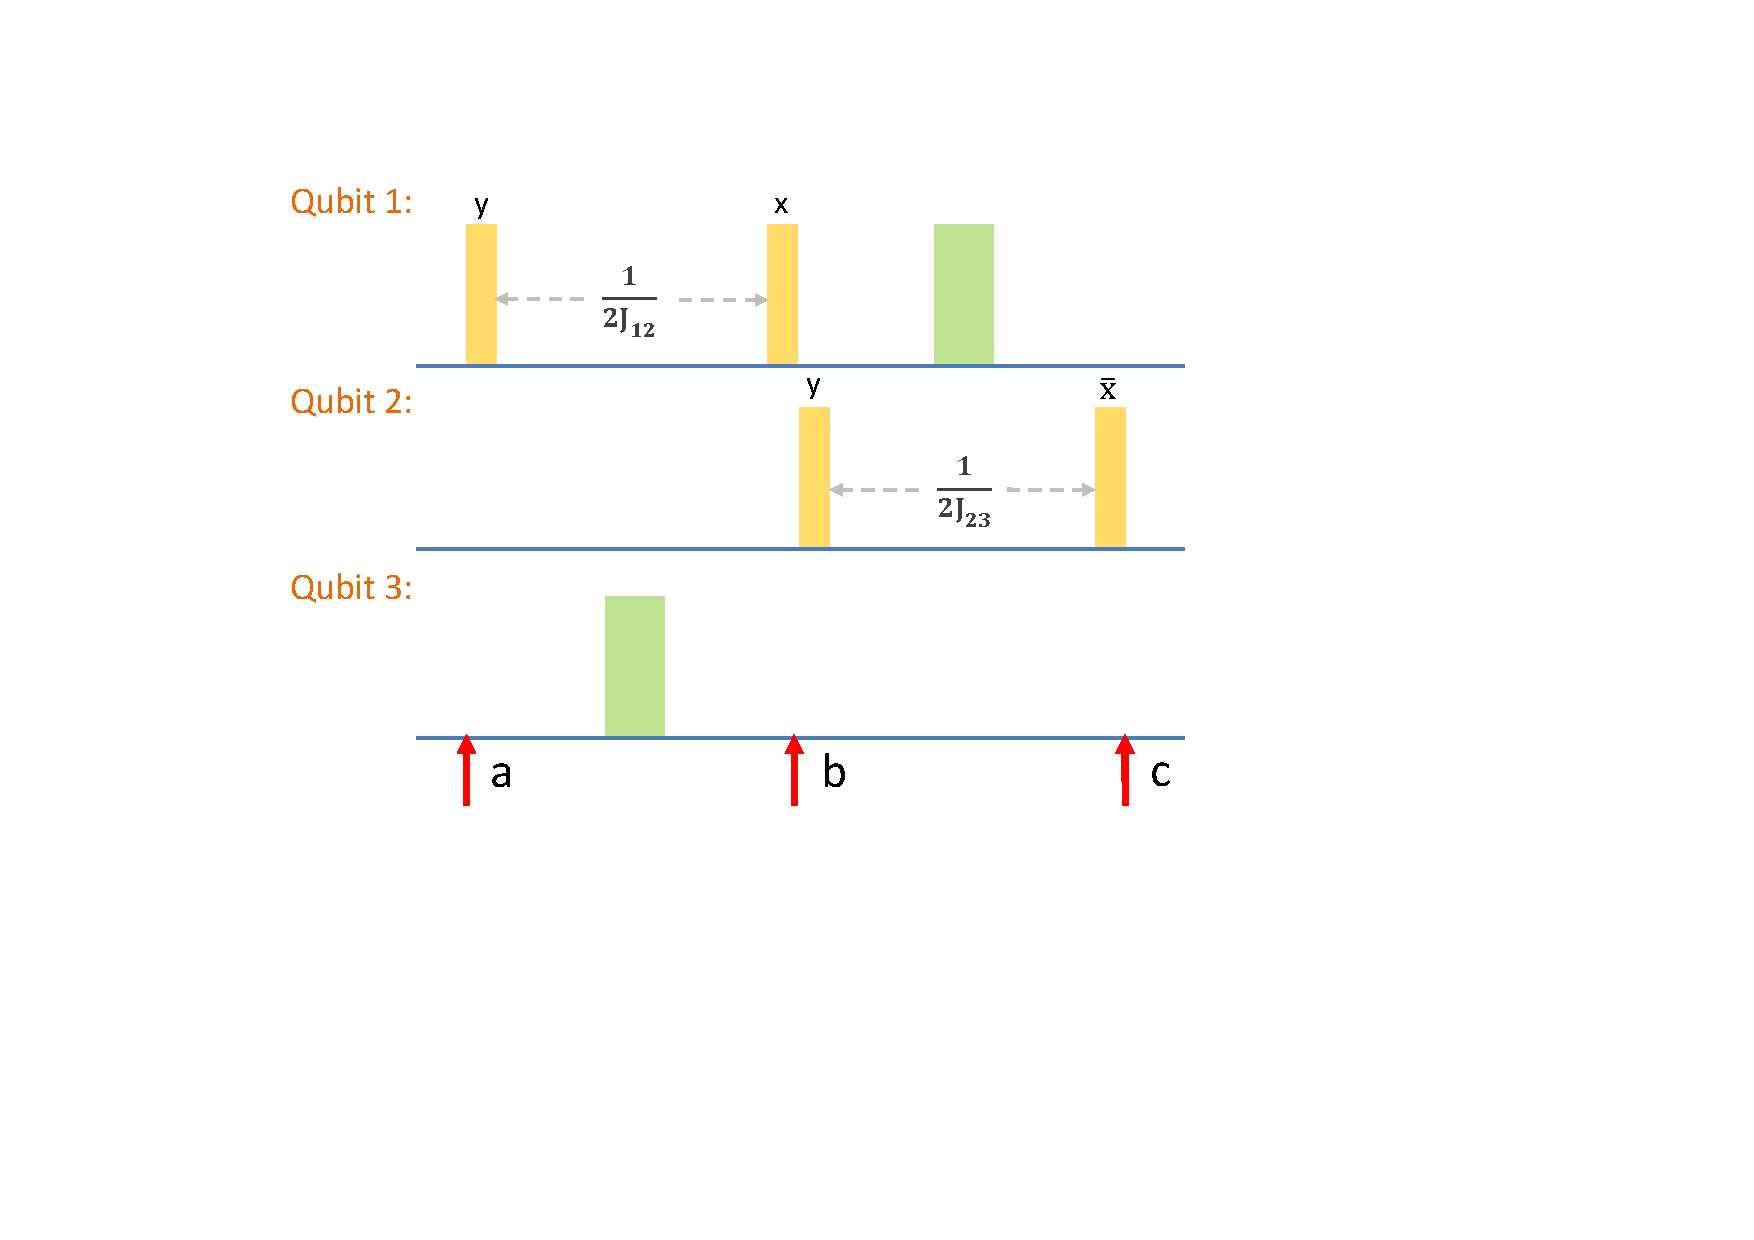
\includegraphics[width=0.9\columnwidth]{1dpulse.pdf}
\caption{Pulse sequence for determining the relative signs of J-couplings}\label{1dpulse}
\end{figure}

At the beginning, the state is prepared to $\rho_a = I_z^1$, which can be easily done by gradient pulses. Under the interaction of $J_{12}$, the state of the system will evolve to $\rho_b = sign(J_{12})2I_z^1I_z^2$. Then $J_{23}$ interaction drives the system to the final state $\rho_c = sign(J_{12})sign(J_{23})4I_z^1I_z^2I_z^3$. The whole procedure is summarized in Fig. \ref{1dpulse}.

\begin{figure}[h] \centering
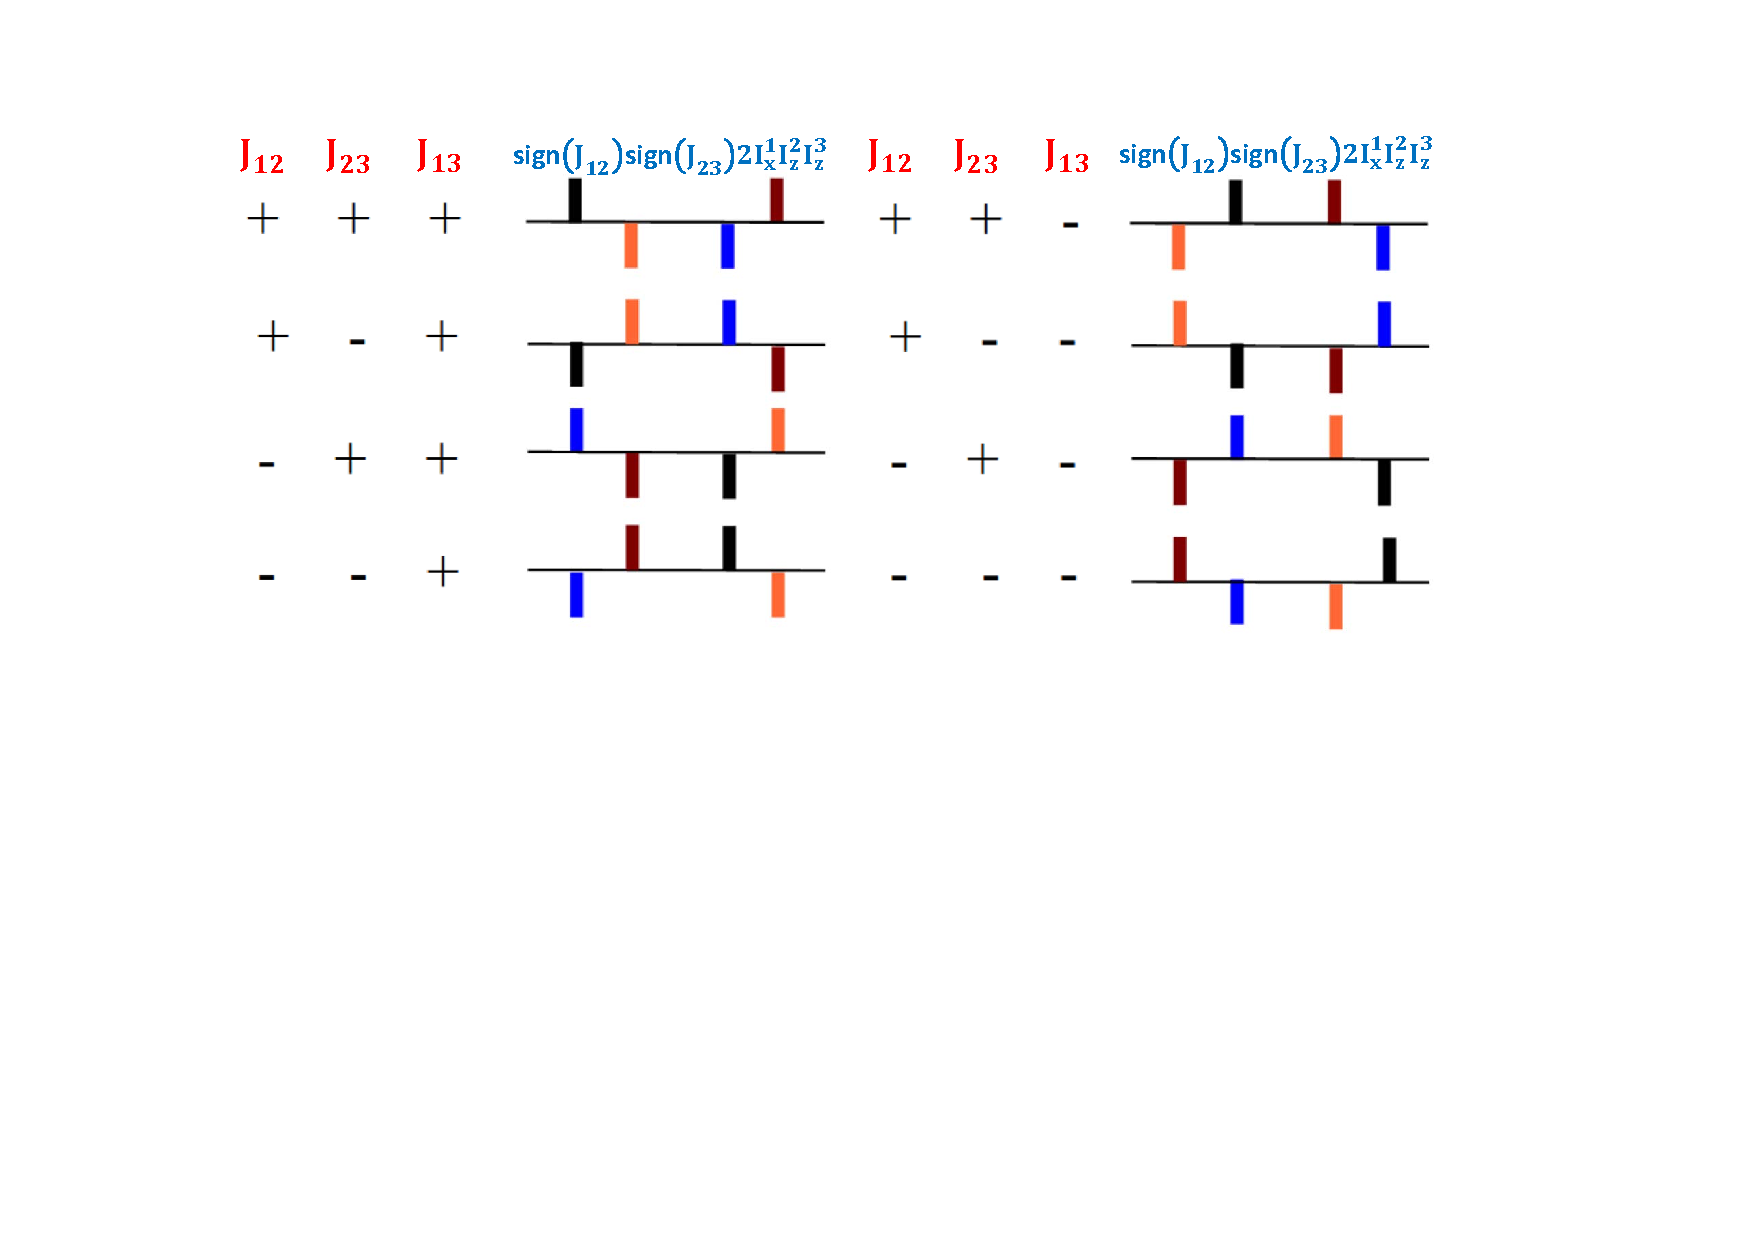
\includegraphics[width=0.9\columnwidth]{1dspectrum.pdf}
\caption{Eight spectra corresponding to the eight different cases.}\label{1dspectrum}
\end{figure}

Assuming $|J_{12}|>|J_{23}|$ and rotating qubit 1 to $I_x$, we could get all the possible eight spectra of $ sign(J_{12})sign(J_{23})4I_x^1I_z^2I_z^3$ corresponding to the signs of the three couplings (Fig. \ref{1dspectrum}). They could be divided into two different types, according to the positions of the positive and negative peaks. Namely, by observing the experimental spectrum $sign(J_{12})sign(J_{23})4I_x^1I_z^2I_z^3$, we can determine that the signs of couplings belong to either type. Thus we confirm that the signs of couplings are one of the four cases in this type. Then, if we rotate qubit 3 to $I_x$, and observe the experimental spectrum $sign(J_{12})sign(J_{23})4I_z^1I_z^2I_x^3$, we can obtain another type similarly. By comparing the former four cases determined by $sign(J_{12})sign(J_{23})4I_x^1I_z^2I_z^3$ and the later four cases determined by
$sign(J_{12})sign(J_{23})4I_z^1I_z^2I_x^3$, the signs of the three couplings are reduced to just two possible situations, and it cannot be done any further because they both have the same relative signs.

In the experiment, we take the group of H$_2$, C$_3$ and H$_3$ denoted as qubit 1, 2 and 3, respectively. The pulse sequence is the one shown in Fig. \ref{1dpulse}, but the $\pi$ pulses for refocusing were applied on qubit 1 and 2 during $J_{12}$ evolution and on qubit 2 and 3 during $J_{23}$ evolution. That is because using the 12-qubit sample we need to refocus all other unexpected couplings. The length of the selective pulse on C$_3$ is 1766us, while the length of H$_2$ and H$_3$ is 21290us. The spectrum of $sign(J_{12})sign(J_{23})4I_x^1I_z^2I_z^3$ is displayed in the upper part of Fig. \ref{H2C3H3}. We can see that the four peaks from left to right are -, +, +, -�� which implies that the signs of $J_{12}$, $J_{23}$ and $J_{13}$ belong to one of the following four: (+, +, -), (+, -, +), (-, +, -) or (-, -, +). Then we observed the spectrum of $sign(J_{12})sign(J_{23})4I_z^1I_z^2I_x^3$, getting that the signs also belong to (-, +, +), (-, -, +), (+, +, -), (+, -, -). By comparing these two spectra we can determine that the signs of $J_{12}$, $J_{23}$ and $J_{13}$ is either (+, +, -) or (-, -, +). Since we have known that $J_{13}$ (the coupling between H$_2$ and H$_3$) is negative, we can claim that $J_{12}$ and $J_{23}$ are both positive.

\begin{figure}[h] \centering
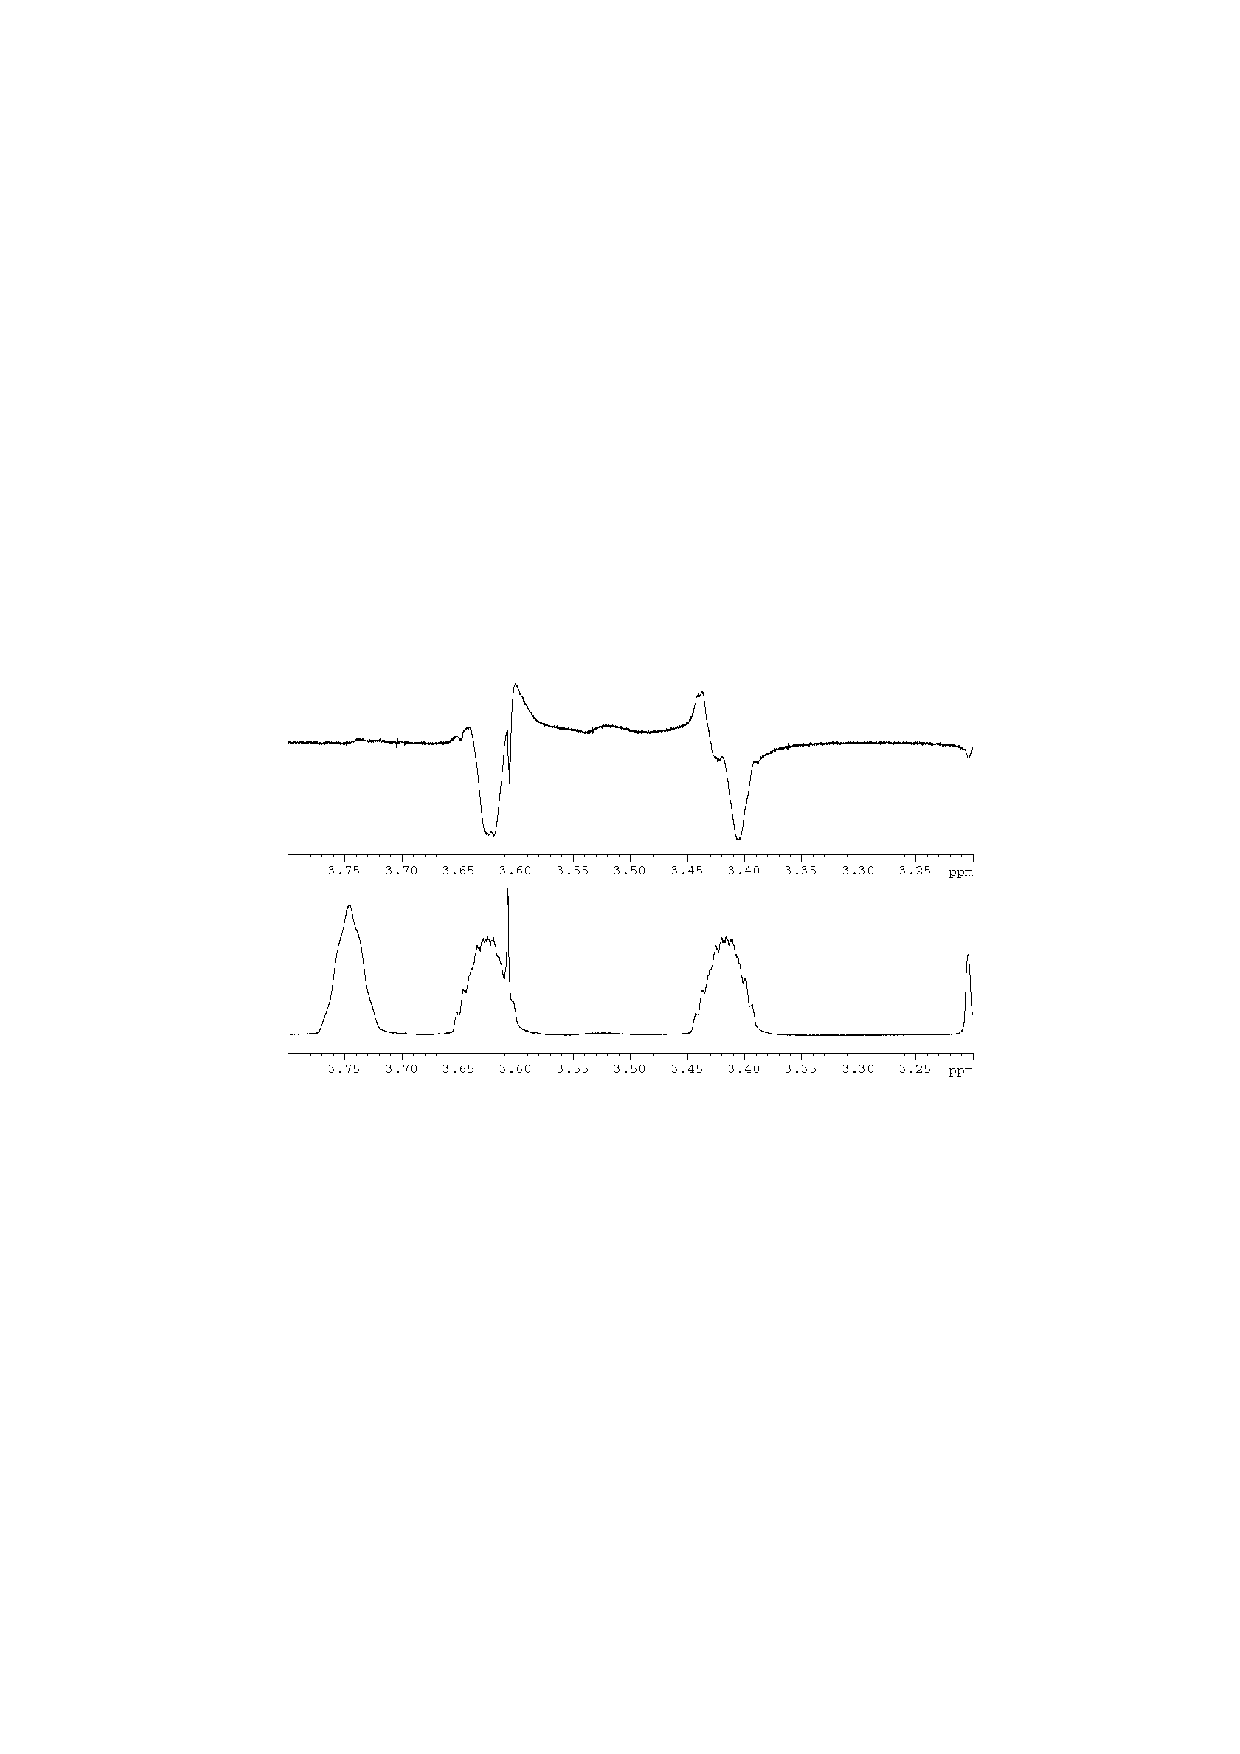
\includegraphics[width=0.9\columnwidth]{H2C3H3.pdf}
\caption{Spectrum of the $sign(J_{12})sign(J_{23})4I_x^1I_z^2I_z^3$ (upper part) and the thermal equilibrium of H$2$ (lower part). The four peaks of the $sign(J_{12})sign(J_{23})4I_x^1I_z^2I_z^3$ from left to right are -, +, +, -. By comparing it to Fig. \ref{1dspectrum}, we can determine that the signs of $J_{12}$, $J_{23}$ and $J_{13}$ belong to one of the following four cases: (+, +, -), (+, -, +), (-, +, -) or (-, -, +)}\label{H2C3H3}
\end{figure}

\subsection{2D MQ experiment}

Theoretically, we could use selective multiple quantum (MQ)- single quantum (SQ) correlation experiment to determine the relative signs of J-couplings, even in the heteronuclear case. Through the pulse sequence (Fig. \ref{mqsequence}), it is comprehensible for this methodology.

\begin{figure}[h] \centering
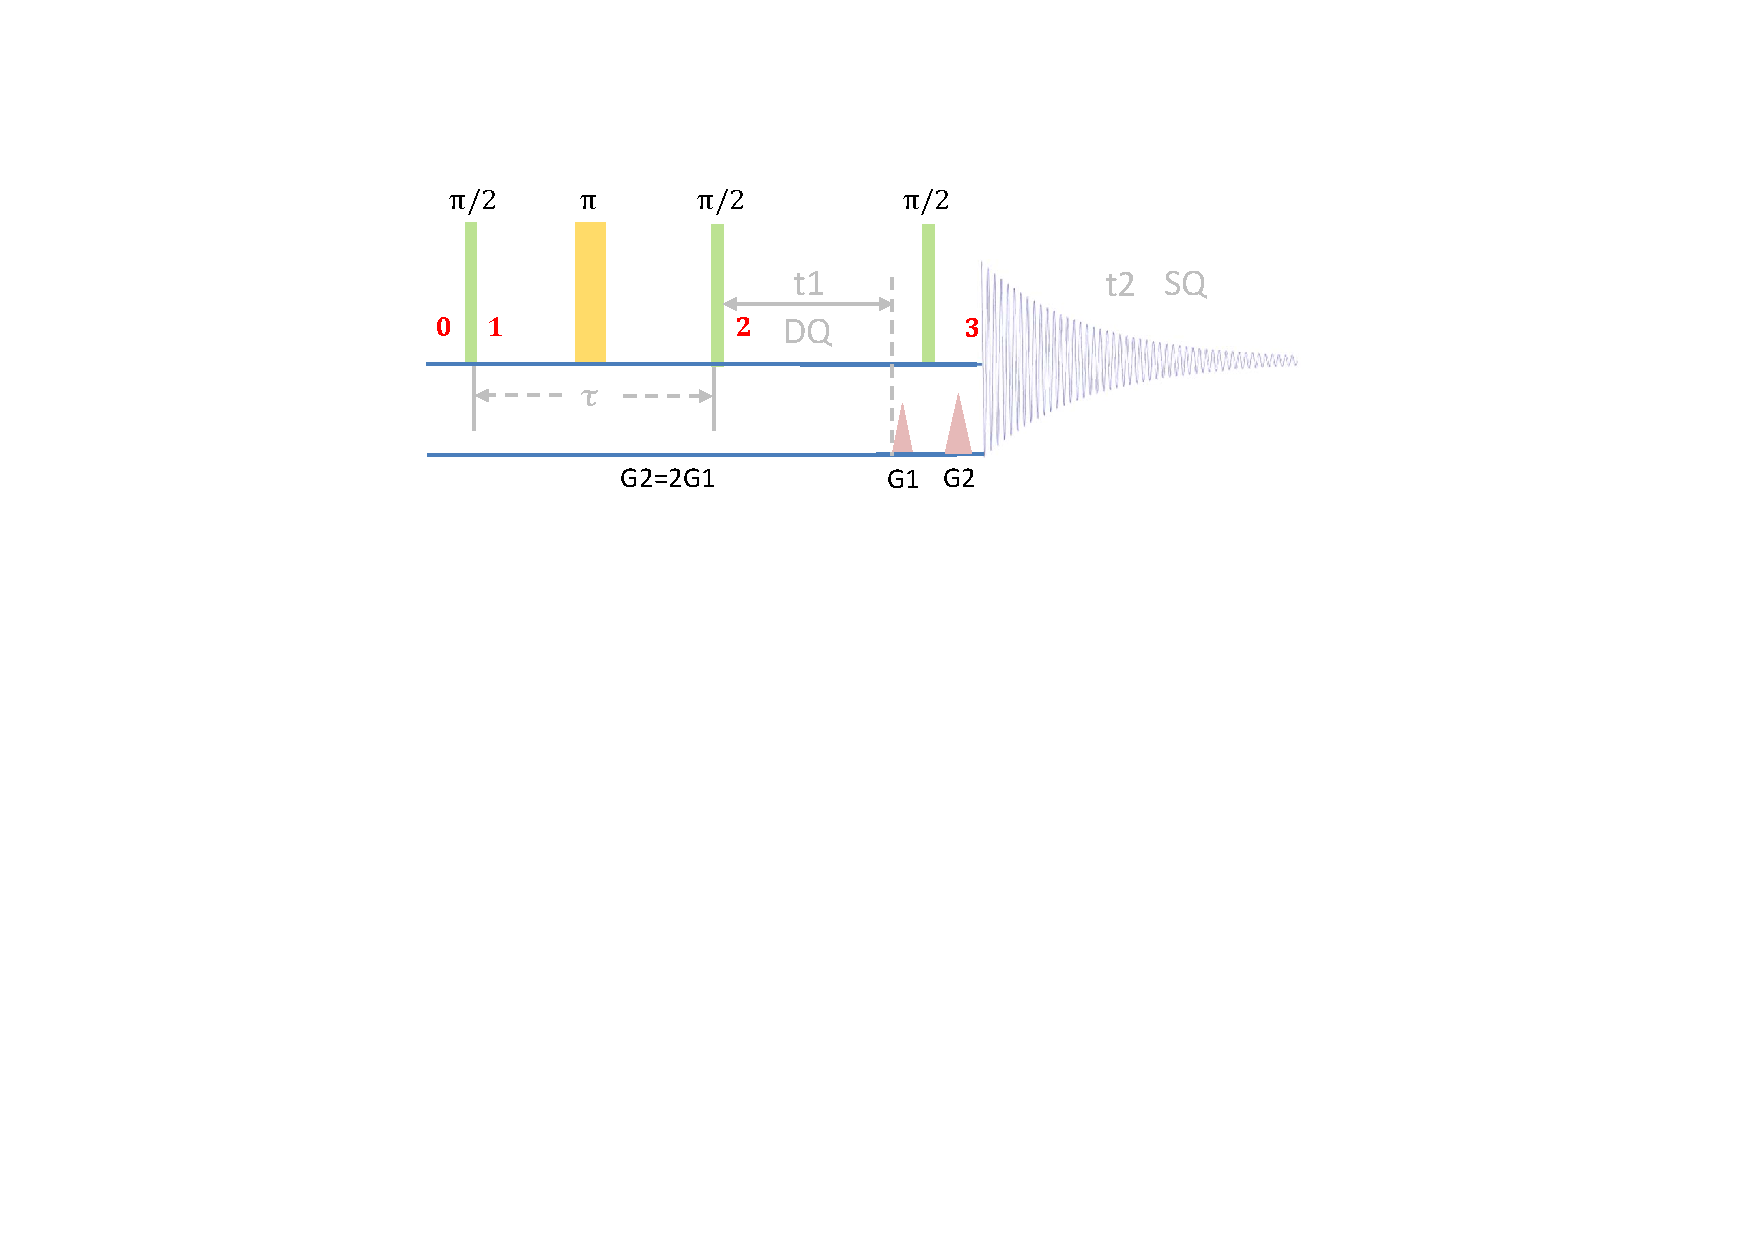
\includegraphics[width=0.9\columnwidth]{mqsequence.pdf}
\caption{Pulse sequence for the $^{13}$C channel. The gradient ration is set to 1:2 to select the DQ coherence.}\label{mqsequence}
\end{figure}

The system considered here is a three spin system, with two $^{13}$C and one $^{1}$H. The internal Hamiltonian is
\begin{eqnarray}\label{2Hamil}
\mathcal{H}_{int}= \omega_1 I_z^1+\omega_2 I_z^2 +\omega_3 I_z^3+ 2\pi J_{12} I_z^1 I_z^2+2\pi J_{13} I_z^1 I_z^3+2\pi J_{23} I_z^2 I_z^3,
\end{eqnarray}
where the subscript 3 stands for the proton. The $\pi$ pulse at the middle of the first two $\pi/2$ pulses ensures the evolution of $J_{12}$.
The second $\pi/2$ pulse converts the antiphase magnetization into double quantum (DQ) coherence. If we choose the evolution time $\tau = 1/2J_{12}$, the current state at point 2 will be $-2(I_x^1I_y^2+I_y^1I_x^2)+I_z^3$. The two gradients before and after the third $\pi/2$ pulse ensure that only the DQ order is selected, while the third $\pi/2$ pulse is using to convert DQ to detectable SQ coherence. The key step of this sequence is the free evolution of $t_1$.

At point 2, the state is $-2(I_x^1I_y^2+I_y^1I_x^2)+I_z^3$. As $I_z^3$ will remain unchanged during $t_1$ and will not affect the spectrum, only the DQ coherence $-DQ_Y = -2(I_x^1I_y^2+I_y^1I_x^2)$ needs to be investigated.

First, the evolution of the chemical shift will transfer the DQ term to
\begin{eqnarray}\label{2Hamil}
-DQ_Y & \rightarrow &-2(I_x^1I_y^2+I_y^1I_x^2)cos(\omega_1t_1+\omega_2t_1) \\ \nonumber
&&-2(I_x^1I_x^2-I_y^1I_y^2)sin(\omega_1t_1+\omega_2t_1).
\end{eqnarray}
Then under the sum of the passive couplings the DQ term will further be converted to
\begin{eqnarray}\label{2Hamil}
\rightarrow &(I_x^1I_y^2+I_y^1I_x^2)cos(\omega_1t_1+\omega_2t_1)cos(\pi J_{13} t_1 +\pi J_{23} t_1) \\ \nonumber
&-2(I_x^1I_x^2-I_y^1I_y^2)I_z^3cos(\omega_1t_1+\omega_2t_1)sin(\pi J_{13} t_1 +\pi J_{23} t_1) \\ \nonumber
&-(I_x^1I_x^2-I_y^1I_y^2)sin(\omega_1t_1+\omega_2t_1)cos(\pi J_{13} t_1 +\pi J_{23} t_1) \\ \nonumber
&-2(I_x^1I_y^2+I_y^1I_x^2)I_z^3sin(\omega_1t_1+\omega_2t_1)sin(\pi J_{13} t_1 +\pi J_{23} t_1).
\end{eqnarray}
After the last $\pi/2$ pulse, the DQ term will be observable
\begin{eqnarray}\label{2Hamil}
\rightarrow &\frac{1}{2}(I_x^1I_z^2+I_z^1I_x^2)[cos(\omega_1+\omega_2+\pi J_{13} +\pi J_{23})t_1 +cos(\omega_1+\omega_2-\pi J_{13} -\pi J_{23})t_1]\\ \nonumber
&+(I_x^1I_x^2-I_z^1I_z^2)I_z^3 [sin(\omega_1+\omega_2+\pi J_{13} +\pi J_{23})t_1 -sin(\omega_1+\omega_2-\pi J_{13} -\pi J_{23})t_1]\\ \nonumber
&-\frac{1}{2}(I_x^1I_x^2-I_z^1I_z^2)I_z^3 [sin(\omega_1+\omega_2+\pi J_{13} +\pi J_{23})t_1 +sin(\omega_1+\omega_2-\pi J_{13} -\pi J_{23})t_1]\\ \nonumber
&+(I_x^1I_z^2+I_z^1I_x^2)I_z^3 [cos(\omega_1+\omega_2+\pi J_{13} +\pi J_{23})t_1 -cos(\omega_1+\omega_2-\pi J_{13} -\pi J_{23})t_1].
\end{eqnarray}
The part that would infect the Fourier Transform of $t_2$ could be analyzed similarly to the text of 2D COSY45 experiment,which is not important in the determination of the signs. However, there are two frequencies in F$_1$ dimension, $\omega_1+\omega_2+\pi J_{13} +\pi J_{23}$  and $\omega_1+\omega_2-\pi J_{13} -\pi J_{23}$.  The difference between them is $2\pi J_{13} +2\pi J_{23}$. If we have known the absolute values of the $ J_{13}$ and $J_{23}$, we could determine the relative signs of them directly.

For a large system, assuming $n_1$ $^{13}$C and  $n_2$ $^{1}$H, we could still use this method. Through the interactions between the passive spins (all the $^{1}$H) and the active spins (all the $^{13}$C), the $n_1$ order coherence will be formed. Therefore the strengths of the gradient fields should be chosen as $G_2 = n_1 G_1$ to select the $n_1$ order coherence. On the F$_1$ dimension of the spectrum we would get all the information of the C-H couplings, and then the relative signs can be determined.


\clearpage

\section{Appendix}

\subsection{Weak J-Coupling Approximation}

Here in this molecule we consider all the J-couplings between any two carbons are weak, which means the J-coupling form is $J_{ij}I_z^iI_z^k$ instead of the strong coupling form $J_{ij}(I_x^iI_x^k+I_y^iI_y^k+I_z^iI_z^k)$. This weak J-coupling approximation depends on the value of
\begin{eqnarray}\label{weak}
tan(2\theta_{ij}) = |J_{ij}/(\nu_i - \nu_j)|,
\end{eqnarray}
where $\nu_i$ and $\nu_j$ are the resonant frequencies of spins $i$ and $j$, respectively. Usually when $tan(2\theta_{ij})\ll 1$, we can say the J-coupling is \emph{weak}, otherwise it should be considered as \emph{strong}. For different types of nuclear spins, such as $^{13}$C and $^{1}$H, the J-couplings will always be weak as in this case the two spins have so different resonant frequencies compared to their coupling. However, for the same type of spins, this value might be much bigger, which means that we cannot apply weak J-coupling approximation. To demonstrate all the J-couplings between carbons are weak, we just need to prove that the J-coupling between the two carbons which have the biggest value of $tan(2\theta)$ can be considered as weak.

In the strong J-coupling case, the Hamiltonian of a 2-qubit system can be written as 
\begin{eqnarray}\label{weak}
H = 2\pi (\nu_1 I_z^1 + \nu_2 I_z^2 + J_{12}I_z^1I_z^2).
\end{eqnarray}
Its eigenvalues and eigenvectors are list as follows (assuming $\nu_1 > \nu_2$ and J is positive):
\begin{eqnarray}\label{2Hamil}
 |00\rangle:&-\frac{1}{2}\nu_1-\frac{1}{2}\nu_2 + \frac{1}{4}J_{12} \\ \nonumber
cos\theta|00\rangle + sin\theta|11\rangle:&+\frac{1}{2}\sqrt{(\nu_1 - \nu_2)^2+J_{12}^2}-\frac{1}{4}J_{12} \\ \nonumber
sin\theta|00\rangle - cos\theta|11\rangle:&-\frac{1}{2}\sqrt{(\nu_1 - \nu_2)^2+J_{12}^2}-\frac{1}{4}J_{12}\\ \nonumber
|11\rangle:&+\frac{1}{2}\nu_1+\frac{1}{2}\nu_2 + \frac{1}{4}J_{12}.
\end{eqnarray}
Then we can calculate the frequencies and intensities of the four peaks in this 2-qubit system 
\begin{eqnarray}\label{strong_peak}
+\frac{1}{2}\nu_1+\frac{1}{2}\nu_2 +\frac{1}{2}\sqrt{(\nu_1 - \nu_2)^2+J_{12}^2} +\frac{1}{2}J_{12}, & \propto (cos\theta-sin\theta)^2  \\ \nonumber
+\frac{1}{2}\nu_1+\frac{1}{2}\nu_2 +\frac{1}{2}\sqrt{(\nu_1 - \nu_2)^2+J_{12}^2} -\frac{1}{2}J_{12}, & \propto (cos\theta+sin\theta)^2\\ \nonumber
+\frac{1}{2}\nu_1+\frac{1}{2}\nu_2 -\frac{1}{2}\sqrt{(\nu_1 - \nu_2)^2+J_{12}^2} +\frac{1}{2}J_{12}, & \propto (cos\theta+sin\theta)^2\\ \nonumber
+\frac{1}{2}\nu_1+\frac{1}{2}\nu_2 -\frac{1}{2}\sqrt{(\nu_1 - \nu_2)^2+J_{12}^2} -\frac{1}{2}J_{12}, & \propto (cos\theta-sin\theta)^2.
\end{eqnarray}
Under the weak J-coupling approximation, the four peaks have the same intensity, and the frequencies are simply $\nu_1\pm\frac{1}{2}J_{12}$ and $\nu_2\pm\frac{1}{2}J_{12}$, respectively. By comparing these two cases we can see that both the frequencies and intensities vary under the weak J-coupling approximation.

By scanning the parameter table of the Hamiltonian, we can find that the maximum value of $tan(2\theta)$ is
\begin{eqnarray}\label{weak}
tan(2\theta_{47}) = |J_{47}/(\nu_4 - \nu_7)|=0.0182,
\end{eqnarray}
where $\nu_4=10333$Hz,  $\nu_7=11928$Hz and $J_{47}=29.02$Hz. If we take the Hamiltonian of C$_4$ and C$_7$ as the strong J-coupling form, we can obtain that the frequencies (intensities) of the four peaks are 
\begin{eqnarray}\label{weak}
11942.64(0.982), 11913.62(1.018), 10347.38(1.018), 10318.36(0.982).
\end{eqnarray}
If we apply the weak J-coupling approximation, the frequencies (intensities) of the four peaks will be
\begin{eqnarray}\label{weak}
11942.51(1), 11913.49(1), 10347.51(1), 10318.49(1).
\end{eqnarray}

It can be seen that these two cases are very similar, which means our weak J-coupling approximation is reliable. Since C$_4$ and C$_7$ have the maximum value of $tan(2\theta)$, we could infer that all the other J-couplings between carbons are also suitable to weak J-coupling approximation.








%\begin{enumerate}
%\item G. Gamow, {\it The Constitution of Atomic Nuclei
%and Radioactivity\/} (Oxford Univ. Press, New York, 1931).
%\item W. Heisenberg and W. Pauli, {\it Zeitschr.\ f.
%Physik\/} {\bf 56}, 1 (1929).
%\end{enumerate}



%\begin{enumerate}
%\bibitem{acknowledge}  The authors thank XXXXX for help. This
%work was supported by National Nature Science Foundation of China, the CAS, and the National Fundamental Research Program 2007CB925200.
%\end{enumerate}




\end{document}




















